\documentclass[12pt,draft]{mitthesis} 

\usepackage{lgrind, braket, amsmath,
  amssymb, bbm, booktabs, subfig, color} 

\usepackage[pdftex]{graphicx}
\usepackage[version=3]{mhchem}

\newcommand{\TODO} [1]{\textcolor{magenta}{\textbf{TODO:} #1}}
\newcommand{\NOTE} [1]{\textcolor{magenta}{[\emph{#1}]}}
\newcommand{\POINT}[1]{\textcolor{magenta}{\textbf{POINT:} #1}}

\newcommand{\rcm}{cm$^{-1}$}
\newcommand{\bigspace}{$
  \;
  $}

\newcommand{\astate}{$
  \tilde{A} \: ^1\!A_u
  $}
\newcommand{\AtoX}{$
  \tilde{A} \: ^1\!A_u 
  \leftarrow 
  \tilde{X} \: ^1\Sigma_g^+
  $}
\newcommand{\StoS}{$
  S_1 \leftarrow S_0
  $}
\newcommand{\microsec}{$\mu$s}

% scientific notation
\newcommand{\e}[1]{\ensuremath{\times 10^{#1}}}

% temperatures
\newcommand{\degrees}{\ensuremath{^\circ}}

% hyphenation
\hyphenation{acetylene}
\hyphenation{Hamiltonian}

\begin{document}

\tableofcontents
\clearpage

\subsubsection*{NOTES}

\clearpage

\setcounter{chapter}{3}
\chapter{SEELEM/LIF spectroscopy of acetylene: Spectral signatures of
  energetically distant doorway levels}

\section{Introduction}

The dynamics of singlet$\sim$triplet coupling in the \AtoX \bigspace
(\StoS) electronic spectrum of acetylene, \ce{C2H2}, have been
extensively studied.  This body of work establishes a heirarchical
model for electronic coupling, which leads to the effects of
intersystem crossing and internal conversion: $S_1 \rightarrow T_3
\rightarrow T_{1,2} \rightarrow S_0$.  Top-tier interactions between
the relatively sparse levels of the $S_1$ and $T_3$ electronic states
are of particular interest because (1) they control coupling to the
remaining electronic states of the molecule and (2) they are primarily
determined by vibrational overlap factors and energy denominators, two
sensitive consequents of the molecule's electronic structure.

% Singlet~triplet coupling in the S_1 state of trans-acetylene is
% mediated by the relatively sparse (0.1 per cm-1) levels of the third
% triplet state, T_3.  When a mediating T_3 level is energetically
% distant from an interacting singlet level, traces of its influence
% appear in the patterns of coupling between the singlet level and the
% dense, local manifold of T_1,2 levels (10 per cm-1).  The method of
% SEELEM spectroscopy is tuned to detect molecules in such second-tier
% eigenstates, being most sensitive to states with about 0.1\% S_1
% character.  Conversely, LIF spectroscopy is sensitive to molecules in
% states with large amounts of S_1 character.

Surface Electron Ejection by Laser-Excited Metastables \cite{sneh89a,
  sneh89b, sneh91, humphrey97} (SEELEM) and LIF spectroscopy are
complementary techniques, which, when used together, can provide
information about $S_1 \sim T_3$ interactions \cite{humphrey97,
  mishra04, altunata00, altunata02}.  \TODO{Finish adapting from
  paper.}  LIF detection is limited to short-lived
($\tau_{radiative}<$ 10 \microsec), strongly fluorescing states, while
SEELEM detection is sensitive only to long-lived ($\tau >$ 300
\microsec) states with vertical electronic excitation above a
threshold energy set by the work function of the metal used as the
SEELEM detector surface. Therefore, SEELEM and LIF detection channels
observe mutually exclusive sets of eigenstates that arise from
spin-orbit mixed $S_1$ and $T_{3,2,1}$ zero-order basis states.
Because SEELEM detection is sensitive to the electronic character of
the molecule, a comparison of simultaneously recorded SEELEM and LIF
spectra reveals features of electronic structure and photochemical
pathways that are invisible via traditional, single-channel
spectroscopic probes such as LIF alone, REMPI, phosphorescence, or
phosphor surface \cite{shi98, campos01, burton72}.

% Information gained from comparison of acetylene SEELEM
% and LIF spectra can yield a mechanistic description of
% singlet$\sim$triplet interaction, and holds promise for describing the
% structure and dynamics of other small polyatomic species \cite{jung07,
%   allen07}.
% SEELEM spectroscopy has
% been used in this effort as a tool to examine $S_1 \sim T_3$ coupling,
% by allowing detection of the local manifold of predominantly $T_{1,2}$
% eigenstates in the region surrounding an \StoS\ transition.

The \emph{trans}-bending mode of $S_1$ acetylene, $\nu_3$, is known to
be an important promoter of singlet$\sim$triplet coupling.  In Zeeman
anticrossing experiments, Dupr\'{e} and coworkers observed a rapid
increase in the anticrossing density, as well as the product
$\rho_{\text{vib}} \braket{H_{st}}$, with energy in $\nu_3$
\cite{dupre91, dupre95b}.  They also observed an single large
singlet$\sim$triplet anticrossing in the $3 \nu_3$ $K_a=0$ level,
%with a zero-field matrix element of 0.29 \rcm,
which was in turn perturbed by many smaller couplings \cite{dupre93}.
These observations led the authors to propose that the
singlet$\sim$triplet dynamics of acetylene in the \astate\ state are
best described by a doorway-mediated mechanism, in which particular
triplet vibrational levels mediate intersystem crossing between the
initially excited $S_1$ bright state and the dense manifold of highly
mixed, dark $T_{1,2}$ states.  Subsequent theoretical and experimental
work confirmed that the coupling doorways were vibrational levels of
the $T_3$ electronic state \cite{vacek96, sherrill96, humphrey97,
  altunata00}.

The $S_1$ $3 \nu_3$ $K_a$=1 level has been heavily studied due to a
local $S_1 \sim T_3$ level crossing at $J \approx 3$.  Spectroscopic
patterns in SEELEM arising from the effects of the local $T_3$
perturber in have been discussed by several authors \cite{humphrey97,
  altunata00, altunata01, mishra04}.  Using vibrational overlap
integrals gained from \emph{ab initio} calculations of the $T_3$
electronic surface, Thom and coauthors were able to exclude all but
several candidate $T_3$ levels as the $3\nu_3$ local perturber
\cite{thom07}.
% \POINT{Overlap between $S_1$ and $T_3$ levels predicted by Bryan and
%   Ryan.  (See p.40 of 1/2007--3/2007 notebook.)}
However, recent observations of an increase in average $T_{1,2}$
electronic character at higher values of $J$ suggest that the local
$T_3$ perturber is not the sole, and perhaps not the primary, doorway
for $3 \nu_3$ \cite{degroot07}.

That an energetically distant doorway, which would be required to have
a correspondingly larger spin-orbit matrix element, may play a role in
coupling $S_1$ $3 \nu_3$ to the $T_{1,2}$ manifold is not altogether
surprising, given the energy region in question.  \emph{Ab initio}
calculations are in agreement that an electronic surface crossing
between the $S_1$ and $T_3$ states is energetically nearby
\cite{ventura03, thom07}.  Such a surface crossing would allow for
strong interactions with several $T_3$ levels in the same energy
region.  It should also play a role in promoting singlet$\sim$triplet
coupling within other $S_1$ levels in the same energy region.  The
$4\nu_3$ level, 1000 \rcm\ higher in energy, is also strongly coupled
to the $T_{1,2}$ manifold, although no obvious local $T_3$ doorway has
been observed \cite{drabbels93, ochi91}.

The energies of the $3 \nu_3$ and $4\nu_3$ levels can therefore be
taken as conservative lower and upper bounds for such an $S_1 \sim
T_3$ ``active'' coupling region.  We turn our attention to other
vibrational levels of $S_1$, which, while in this critical energy
region, are not near-degenerate with a mediating $T_3$ level at low
$J$.  The levels chosen for study all lie within 500 \rcm\ of $3
\nu_3$ $K_a$=1, and involve excitation in the Franck-Condon active
modes of $S_1$ acetlyene, $\nu_2$ (C-C stretch) and $\nu_3$
(\emph{trans} bend), with one exception.

In the absence of a local $T_3$ perturber, coupling between $S_1$
levels and the local manifold of $T_{1,2}$ states is expected to be
mediated by energetically distant $T_3$ levels.  Evidence for
energetically distant, mediating $T_3$ levels is obtained by comparing
simultaneously recorded LIF and SEELEM spectra.  Additionally, a new
technique for comparison is developed that is sensitive to the
presence of distant $T_3$ doorway levels.  This new technique takes
into account shifting intensity patterns in the frequency-domain LIF
spectrum as a function of delay time, due to the time development of
an incoherent ensemble of eigenstates with different fluorescence
lifetimes.  When used on a segment of spectrum that includes just one
singlet rovibronic transition, the technique reveals a
coupling-dependent shift in the statistical properties of the spectrum
with delay time.  Comparison with other transitions in a rotational
series can reveal local perturbations caused by weakly coupled $T_3$
levels.  When used on a spectrum containing several rovibronic
transitions in series, the technique can give insight into the matrix
element and relative energy of a $T_3$ doorway level.

\section{COMMUNICATION: Signatures of doorway-mediated intersystem
  crossing in delayed, incoherent fluorescence measurements}

In Chapter 2, we introduced the concept of a SEELEM intensity
distribution associated with one singlet bright state.  

Here, we extend the idea of dark state intensity distributions to
fluorescence measurements by considering intensities in the
\emph{incoherent, frequency domain} LIF spectrum with a time window
$t$ to $t+dt$ after excitation of the molecule.  The SEELEM spectrum
is shown to be a limiting case of delayed fluorescence.  Furthermore,
we demonstrate that molecular properties, such as the spin-orbit
matrix element and the energy denominator for a doorway state, are
revealed by changes in statistical properties of the spectrum as the
time window is shifted from sub-\microsec\ gated LIF, into delayed
LIF, and finally to SEELEM.

\TODO{Adapt following from delayedfluorescence report.}  For a pure
singlet bright state, $\ket{s}$, the time-dependent fluorescence
intensity is
\begin{equation}
  I_s(t) = \frac{1}{\tau_s} \;
           \exp \left[
             -\frac{t}{ \tau_s} 
           \right],
\end{equation}
normalized such that $\int_0^{\infty} I_s(t) \, dt = 1$.

We consider the case where $\ket{s}$ is admixed into a set of $N$
triplet dark states to create a set of $N$+1 mixed states
$\lbrace\ket{m}\rbrace$.  Each mixed state, $\ket{m}$, has some bright
state amplitude $a_m$.  In the case of direct or doorway-mediated
coupling, the Hamiltonian contains only one pathway from each dark
state to the bright state (see Chapter 3).  As a result, all of the
mixing amplitudes may be taken to be real and positive.  If the
lifetime of a pure triplet dark state is much longer than $\tau_s$,
the lifetime of a mixed eigenstate $\ket{m}$ having bright state
fractional character $\alpha_m^2$ is
\begin{equation}
  \label{eq:tau-m}
  \tau_m = \tau_s / a_m^2,
\end{equation}
and its time-dependent fluorescence intensity is
\begin{equation}
  \label{eq:int-m}
  I_m(t) = \frac{a_m^4}{\tau_s} \;
           \exp \left[
             -\frac{a_m^2 \, t}{\tau_s} 
           \right].
\end{equation}
The total integrated fluorescence intensity for a mixed state is
$\int_0^{\infty} I_m(t) \, dt = a_m^2$, relative to unit intensity for
a pure bright state.  This reflects the $a_m^2$ times smaller
probability for excitation of the $\ket{m}$ state.

% The normalization condition for bright state character $\sum_m a_m^2 =
% 1$ leads to the relation
% \begin{equation}
%   \tau_s^{-1} = \sum_m \tau_m^{-1};
% \end{equation}
% in this way, $\tau_s$ can be derived from the set of mixed state
% lifetimes $\lbrace \tau_m \rbrace$.

\subsection{An incoherent, high-resolution fluorescence spectrum after
  a time delay}

We examine the fluorescence intensity after a time delay $t$,
which we cast in units of the bright state lifetime:
\begin{equation}
  R = t / \tau_s.
\end{equation}
At a chosen value of $R$, the fluorescence intensity equation
\ref{eq:int-m} has a single maximum with respect to fractional bright
state character.  \TODO{Insert relevant minmax equation.}
\TODO{Reword: when $R<2$, when $R<2$...} Within the range $0 \le a_m^2
\le 1$, the fluorescence intensity equation is maximized when the
mixing fraction is (Chapter 2, equation 31)
\begin{equation}
  \label{eq:am-max}
  a_m^2 = \frac{2}{R}.
\end{equation}

\begin{figure}
  \caption{The intensity of a mixed eigenstate at time $R =
    t/\tau_s$, plotted as a function of bright
    state character.}
  \label{fig:int-at-rc}
  \centering
  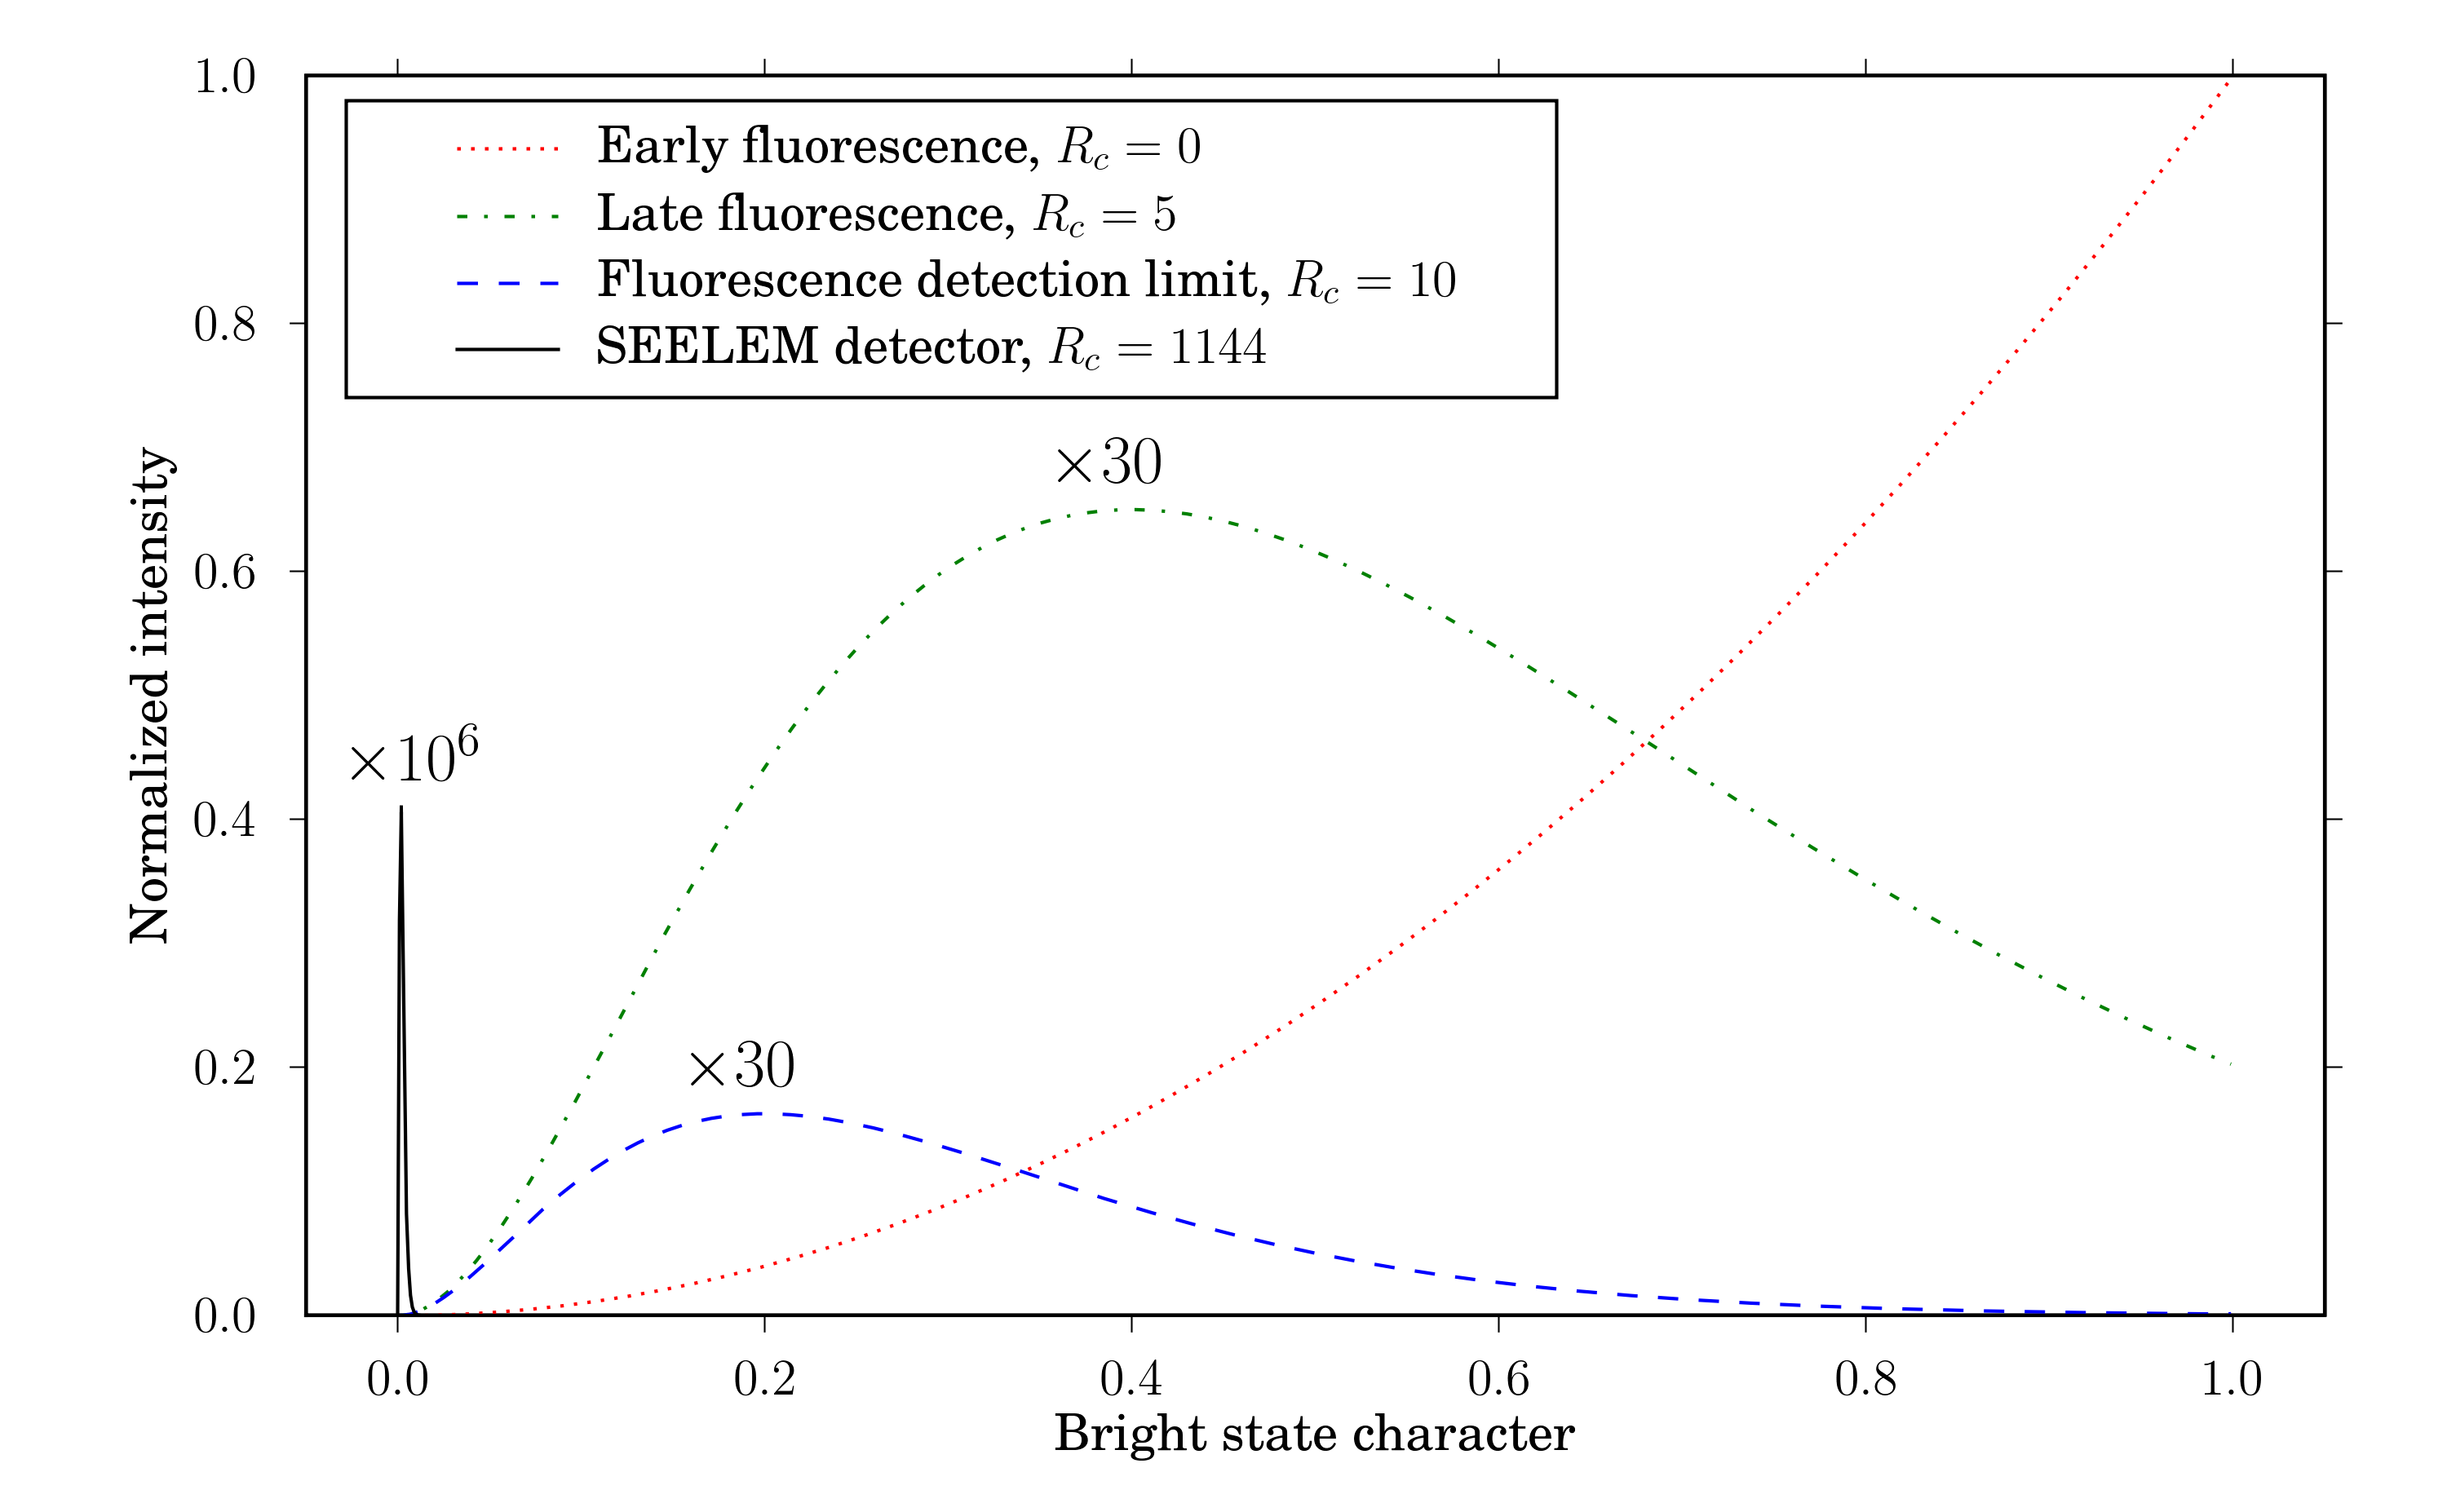
\includegraphics[width=7.5in,angle=90]{intensity-at-rc.png}
\end{figure}

Figure \ref{fig:int-at-rc} shows the dependence of fluorescence
intensity on fractional bright state character at several selectable
values of $R$.  At early fluorescence window times ($t \sim \tau_s$),
the fluorescence intensity is greatest for states with large amounts
of fractional bright state character ($2/R > 1$).  At a delay of $t =
R \tau_s = 5 \tau_s$, the fluorescence intensity equation
discriminates against states with large fractional bright state
character, since molecules in such states have already fluoresced with
high probability.  States with small fractional bright state character
are also discriminated against.  Molecules in such states have a low
probability of fluorescing in the time window under consideration.
The detectable fluorescence intensity may thus be ``tuned'' to a
chosen value of fractional bright state character merely by selecting
a time delay $R$, according to Equation \ref{eq:am-max}.

\POINT{Remove this paragraph?}  Note that the intensity expression
used here does not account for molecules moving out of the field of
view of the fluorescence detection optics.  We consider only the
distribution of bright state character \emph{among molecules that
  remain within the field of view at time $R$}.  However, since there
is no momentum transfer from the excitation photon to the molecule,
the rate of molecules exiting the field of view is independent of
bright state character.  Thus, the statistical properties of the
spectrum in the frequency domain, involving only fluorescence
intensity ratios between molecules with differing fractional bright
state character, are undistorted by molecules moving out of the field
of view.

\TODO{Move this to beginning.}  For the $S_1$ electronic state of
acetylene, $\tau_s=270$ ns \cite{ochi91}.  The field-of-view of the
fluorescence detection optics is about 5 mm, which amounts to a
maximum viewing time of about 5 $\mu$s, about $18\tau_s$, for
molecules in the molecular beam, which has an average velocity of
$10^3$ m/s.  At times later than $10\tau_s$, no molecules remain
within the fluorescence field of view.  This places an upper limit on
the value of $R$ that can be selected in our fluorescence experiments.
Figure \ref{fig:int-at-rc} shows the intensity equation for the long
time limit of fluorescence detection, $18\tau_s$.

The SEELEM detector used in our experiments detects metastable
molecules after a 309 $\mu$s flight time.  If we set aside some
aspects of SEELEM detectivity and consider only its detection
sensitivity to bright state character, we arrive at the following
equation for SEELEM detection probability (Chapter 2, equation 28):
\begin{equation}
  \label{eq:seelem-prob-s}
  P_{SEELEM}^{(s)} \propto a_m^4 \; \exp \left( -R_c \, a_m^2 \right).
\end{equation}
(This is a good approximation to the overall detection sensitivity of
SEELEM, including electron ejection probability resulting from
fractional $T_3$ electronic character, in the weak coupling limit.)
The SEELEM detection probability equation above has the same
functional form as Equation \ref{eq:int-m}.  Thus, the SEELEM detector
may be viewed in this limited sense as an extreme discriminator for
detecting states with small fractional bright state character.

Acetylene molecules in our apparatus are detected after an average
flight time of 309 $\mu$s, yielding an $R_c$ value of $1144$ for the
SEELEM detector.  This corresponds to a maximum detection probability
for states with $0.17\%$ bright state character.

\subsection{Delayed fluorescence of a model system}

Our next step is to examine how the characteristics of a
fluorescence intensity distribution change as we increase the time delay
$R$.  We model the interaction between a bright state and an
ensemble of dark states by generalizing from a two-level system.
Consider a Hamiltonian with only one dark state.  Define the two mixed
states $\ket{m=1,2}$ as
\begin{equation}
  \begin{split}
    \ket{1} &=  (1 - \alpha^2)^{1/2} \ket{s} + \alpha \ket{t}\\
    \ket{2} &= -\alpha \ket{s} + (1 - \alpha^2)^{1/2} \ket{t}.
  \end{split}
\end{equation}
The fluorescence intensity of both states, relative to a pure bright
state, is
\begin{equation}
  \begin{split}
    I_1 &= \frac{(1 - \alpha^2)^2}{\tau_s} \; \exp 
          \left[
            - R \, (1 - \alpha^2)
          \right]\\
    I_2 &= \frac{\alpha^4}{\tau_s} \; \exp 
          \left[
            - R \, \alpha^2
          \right],
  \end{split}
\end{equation}
and the ratio of the fluorescence intensities changes with time,
$t=R\tau_s$, as
\begin{equation}
  I_{12} = I_1 / I_2 = 
  \left(
    \frac{(1 - \alpha^2)}{\alpha^2}
  \right)^2
  \exp
  \left[
    - R \, (1 - 2\alpha^2)
  \right].
\end{equation}  \TODO{Explain behavior of this equation.  Prefactor
  determines initial ratio.  Long time limit, always approaches zero.}

\TODO{Rwrite this -- frame center of gravity in terms of intensity
  ratios.  Explain center of gravity.}  The fluorescence intensity
ratio may be incorporated into an equation for the dependence of
average detected intensity on $R$,
\begin{equation}
  \label{eq:ratio}
  \braket{I_{LIF}} = 
  \frac{\Delta E_{12}}{2} \,
  \left(
    \frac{I_{12}-1}{I_{12}+1}
  \right).
\end{equation}
Figure \ref{fig:ratio} shows the dependence of the intensity-weighted
center-of-gravity on the intensity ratio $I_{12}$.

\begin{figure}
  \caption{Center of gravity as a function of the intensity ratio
    $I_1$:$I_2$ for a two-state system.  At $t=0$, the initial center
    of gravity is a function of the mixing amplitude $\alpha$.  The
    center of gravity then shifts with the changing intensity ratio as
    delay time is increased, arriving at a limiting value of $-\Delta
    E_{12}/2$.}
  \label{fig:ratio}
  \centering
  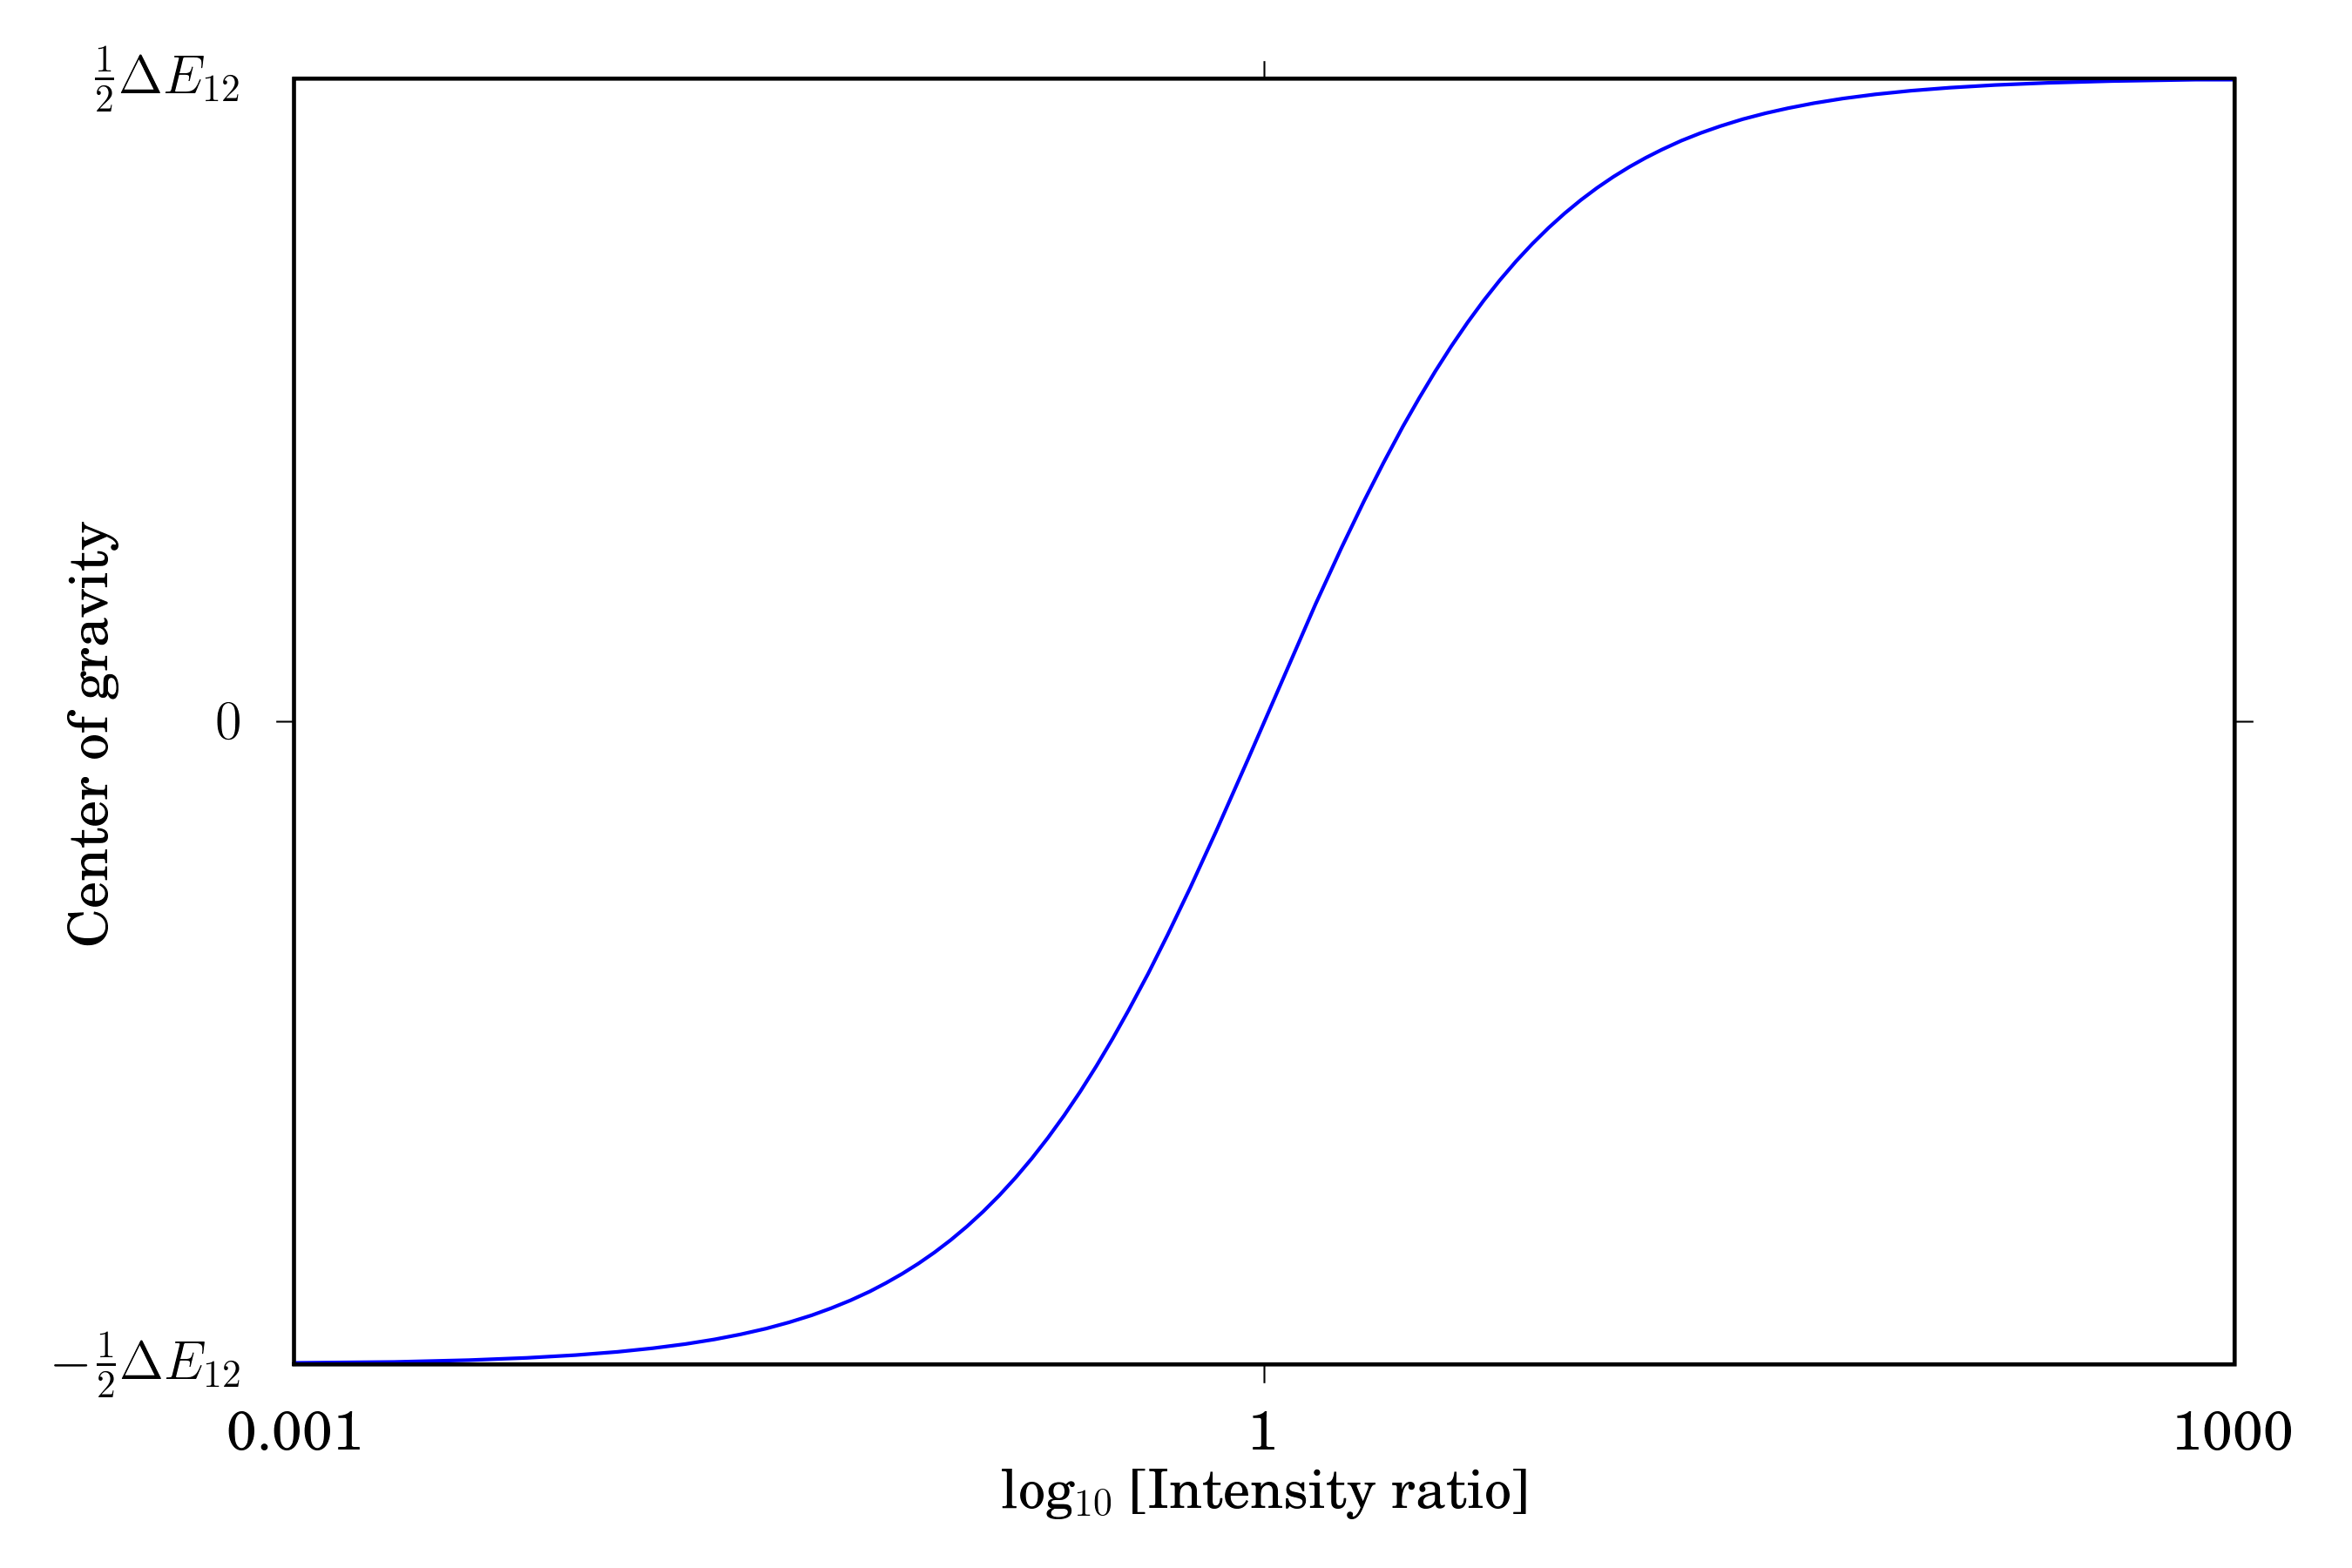
\includegraphics[width=6in]{cog-from-ratio.png}
\end{figure}

The initial intensity ratio at time $R_c=0$ is
\begin{equation}
  I_{12} = 
  \left(
    \frac{(1 - \alpha^2)}{\alpha^2}
  \right)^2.
\end{equation}
From this, the initial center of gravity can be found according to
Equation \ref{eq:ratio} or Figure \ref{fig:ratio}.  At large values of
$R_c$, the intensity ratio decreases to zero as $I_1 \ll I_2$, if the
states are not 50:50 mixed.  As the ratio decreases toward zero, the
intensity-weighted center of gravity approaches $-\Delta E_{12} / 2$.
The R-dependence of intensity ratios and the consequent shift in
center of gravity are shown in Figure \ref{fig:cog-devel}.  

\TODO{Say this more clearly.  Explain weak and strong limits.} One
interesting aspect of the center of gravity shift shown in Figure
\ref{fig:cog-devel} is the sudden onset of the shift at small mixing
coefficients.

\begin{figure}
  \caption{(Top) Time development of the intensity ratio for
    a two state system. (Bottom) Time development of the center of
    gravity for a two state system.}
  \label{fig:cog-devel}
  \centering
  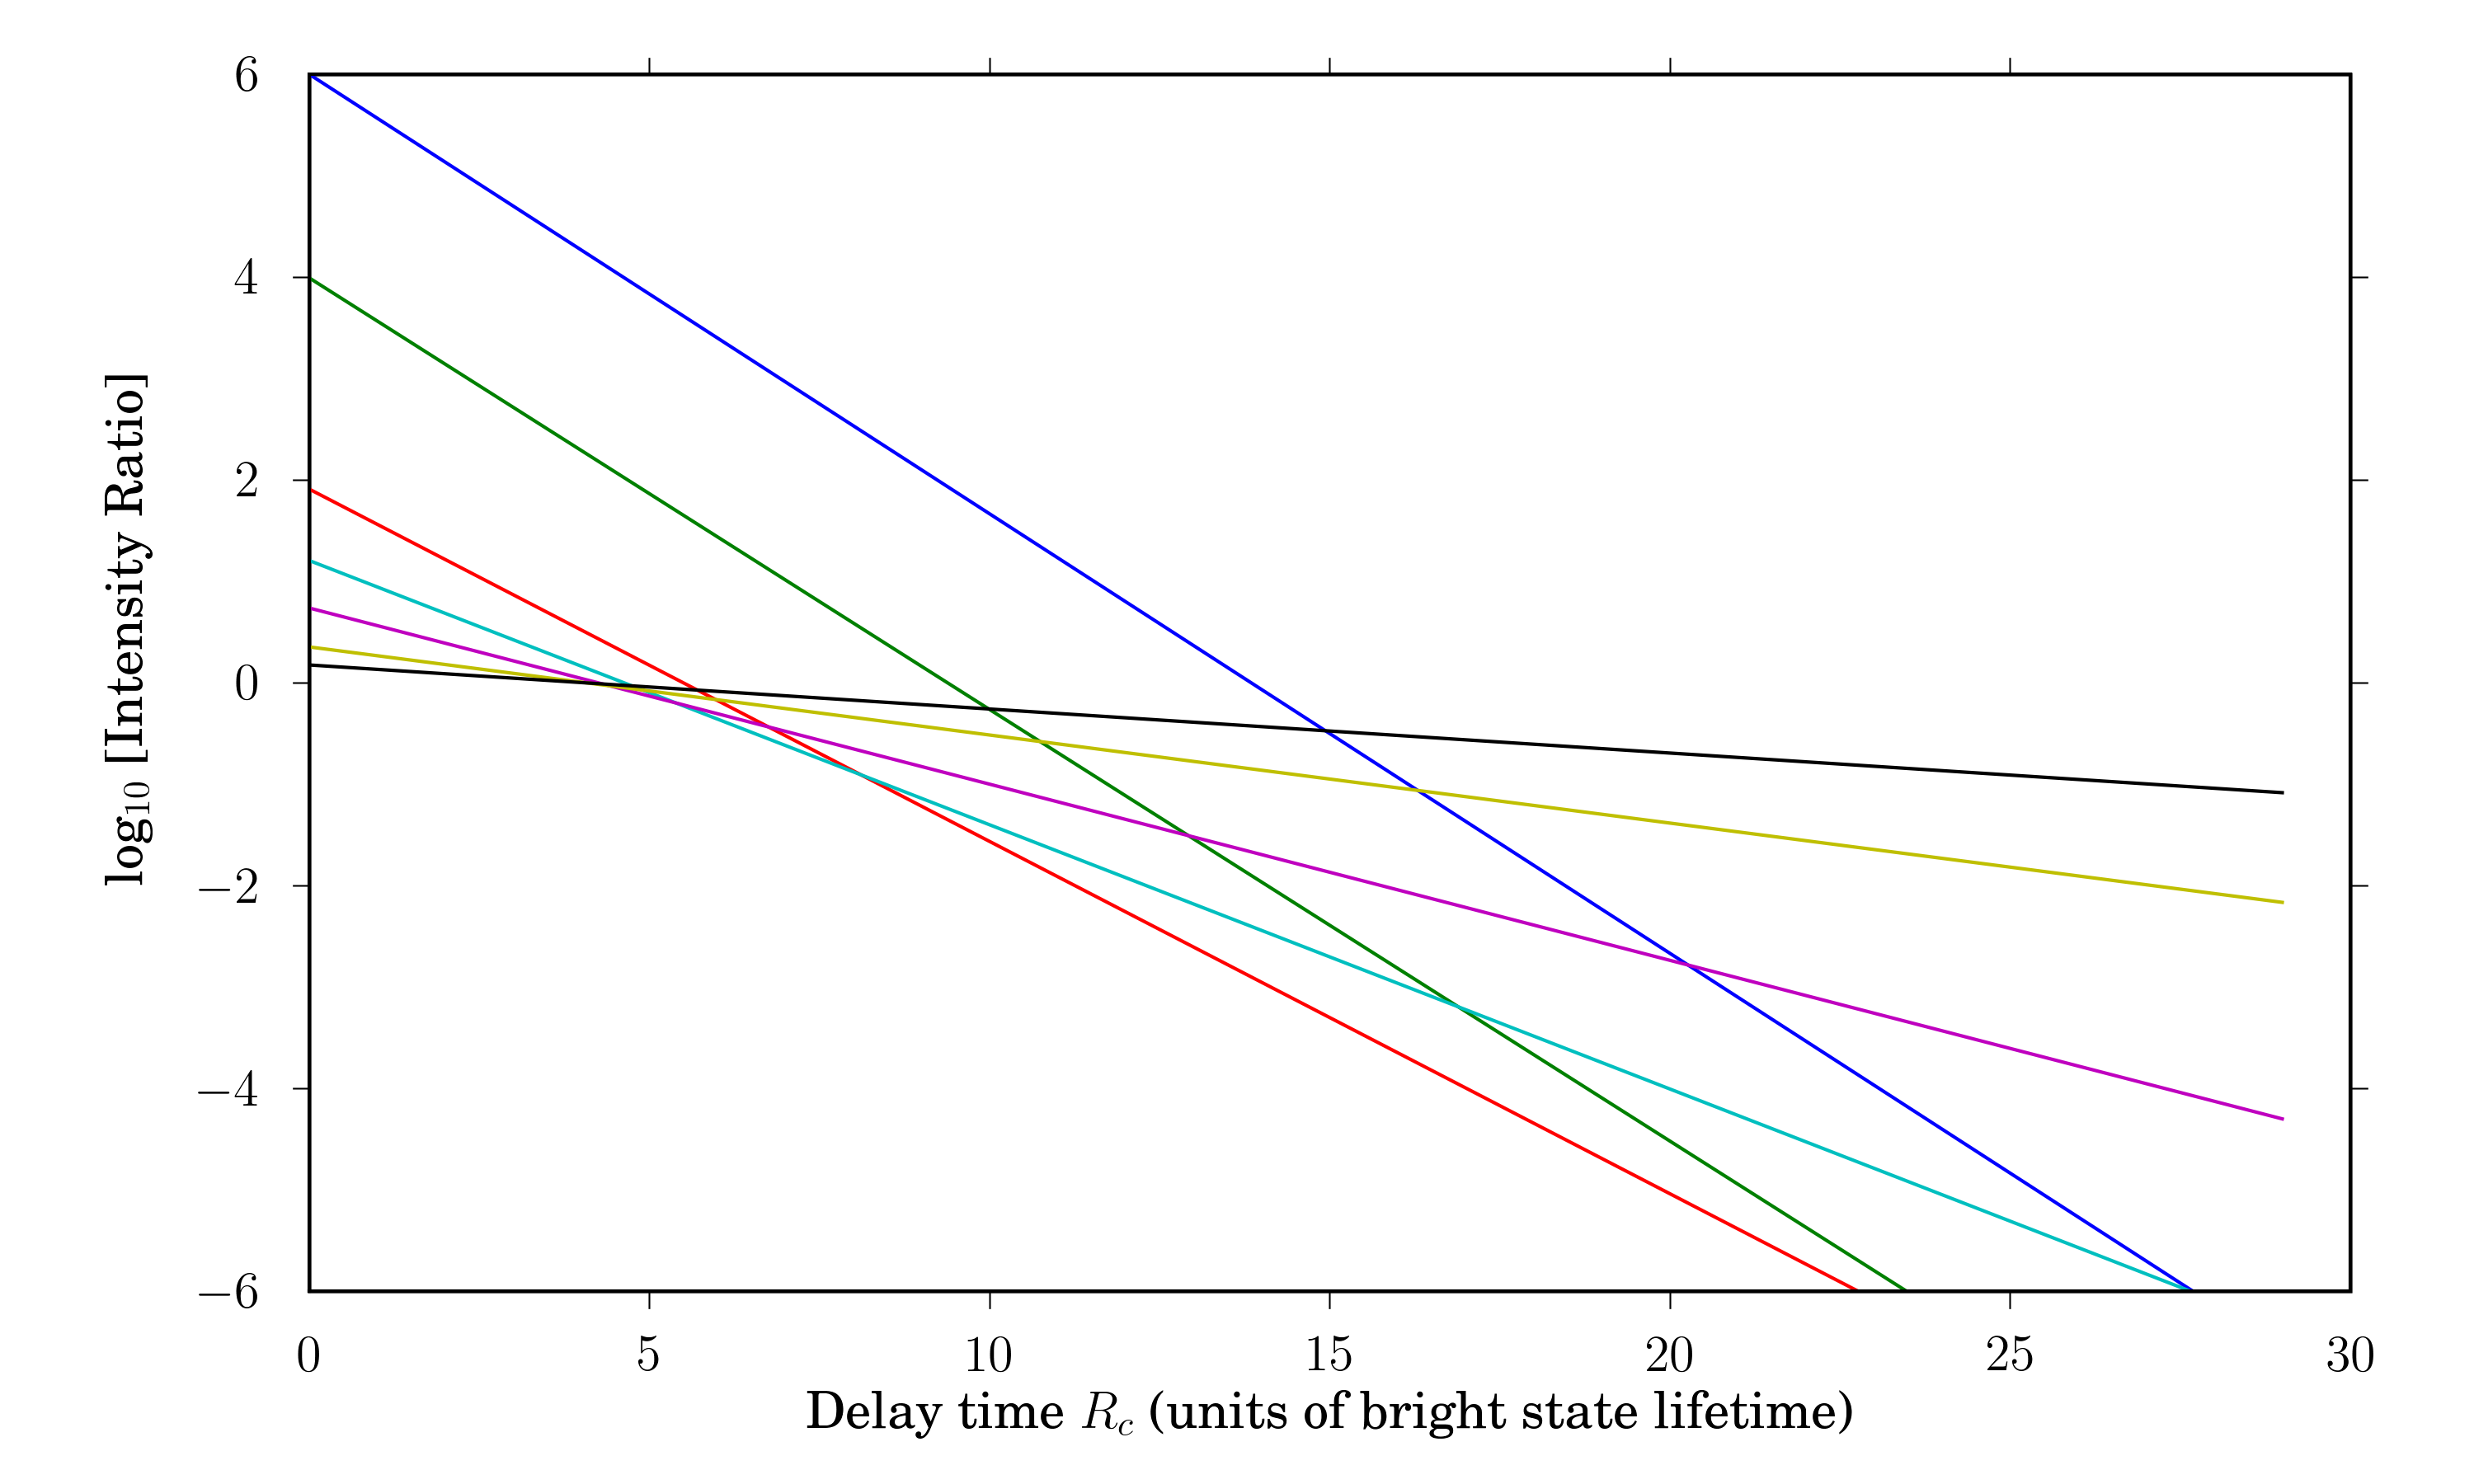
\includegraphics[width=6in]{ratio-development.png}
  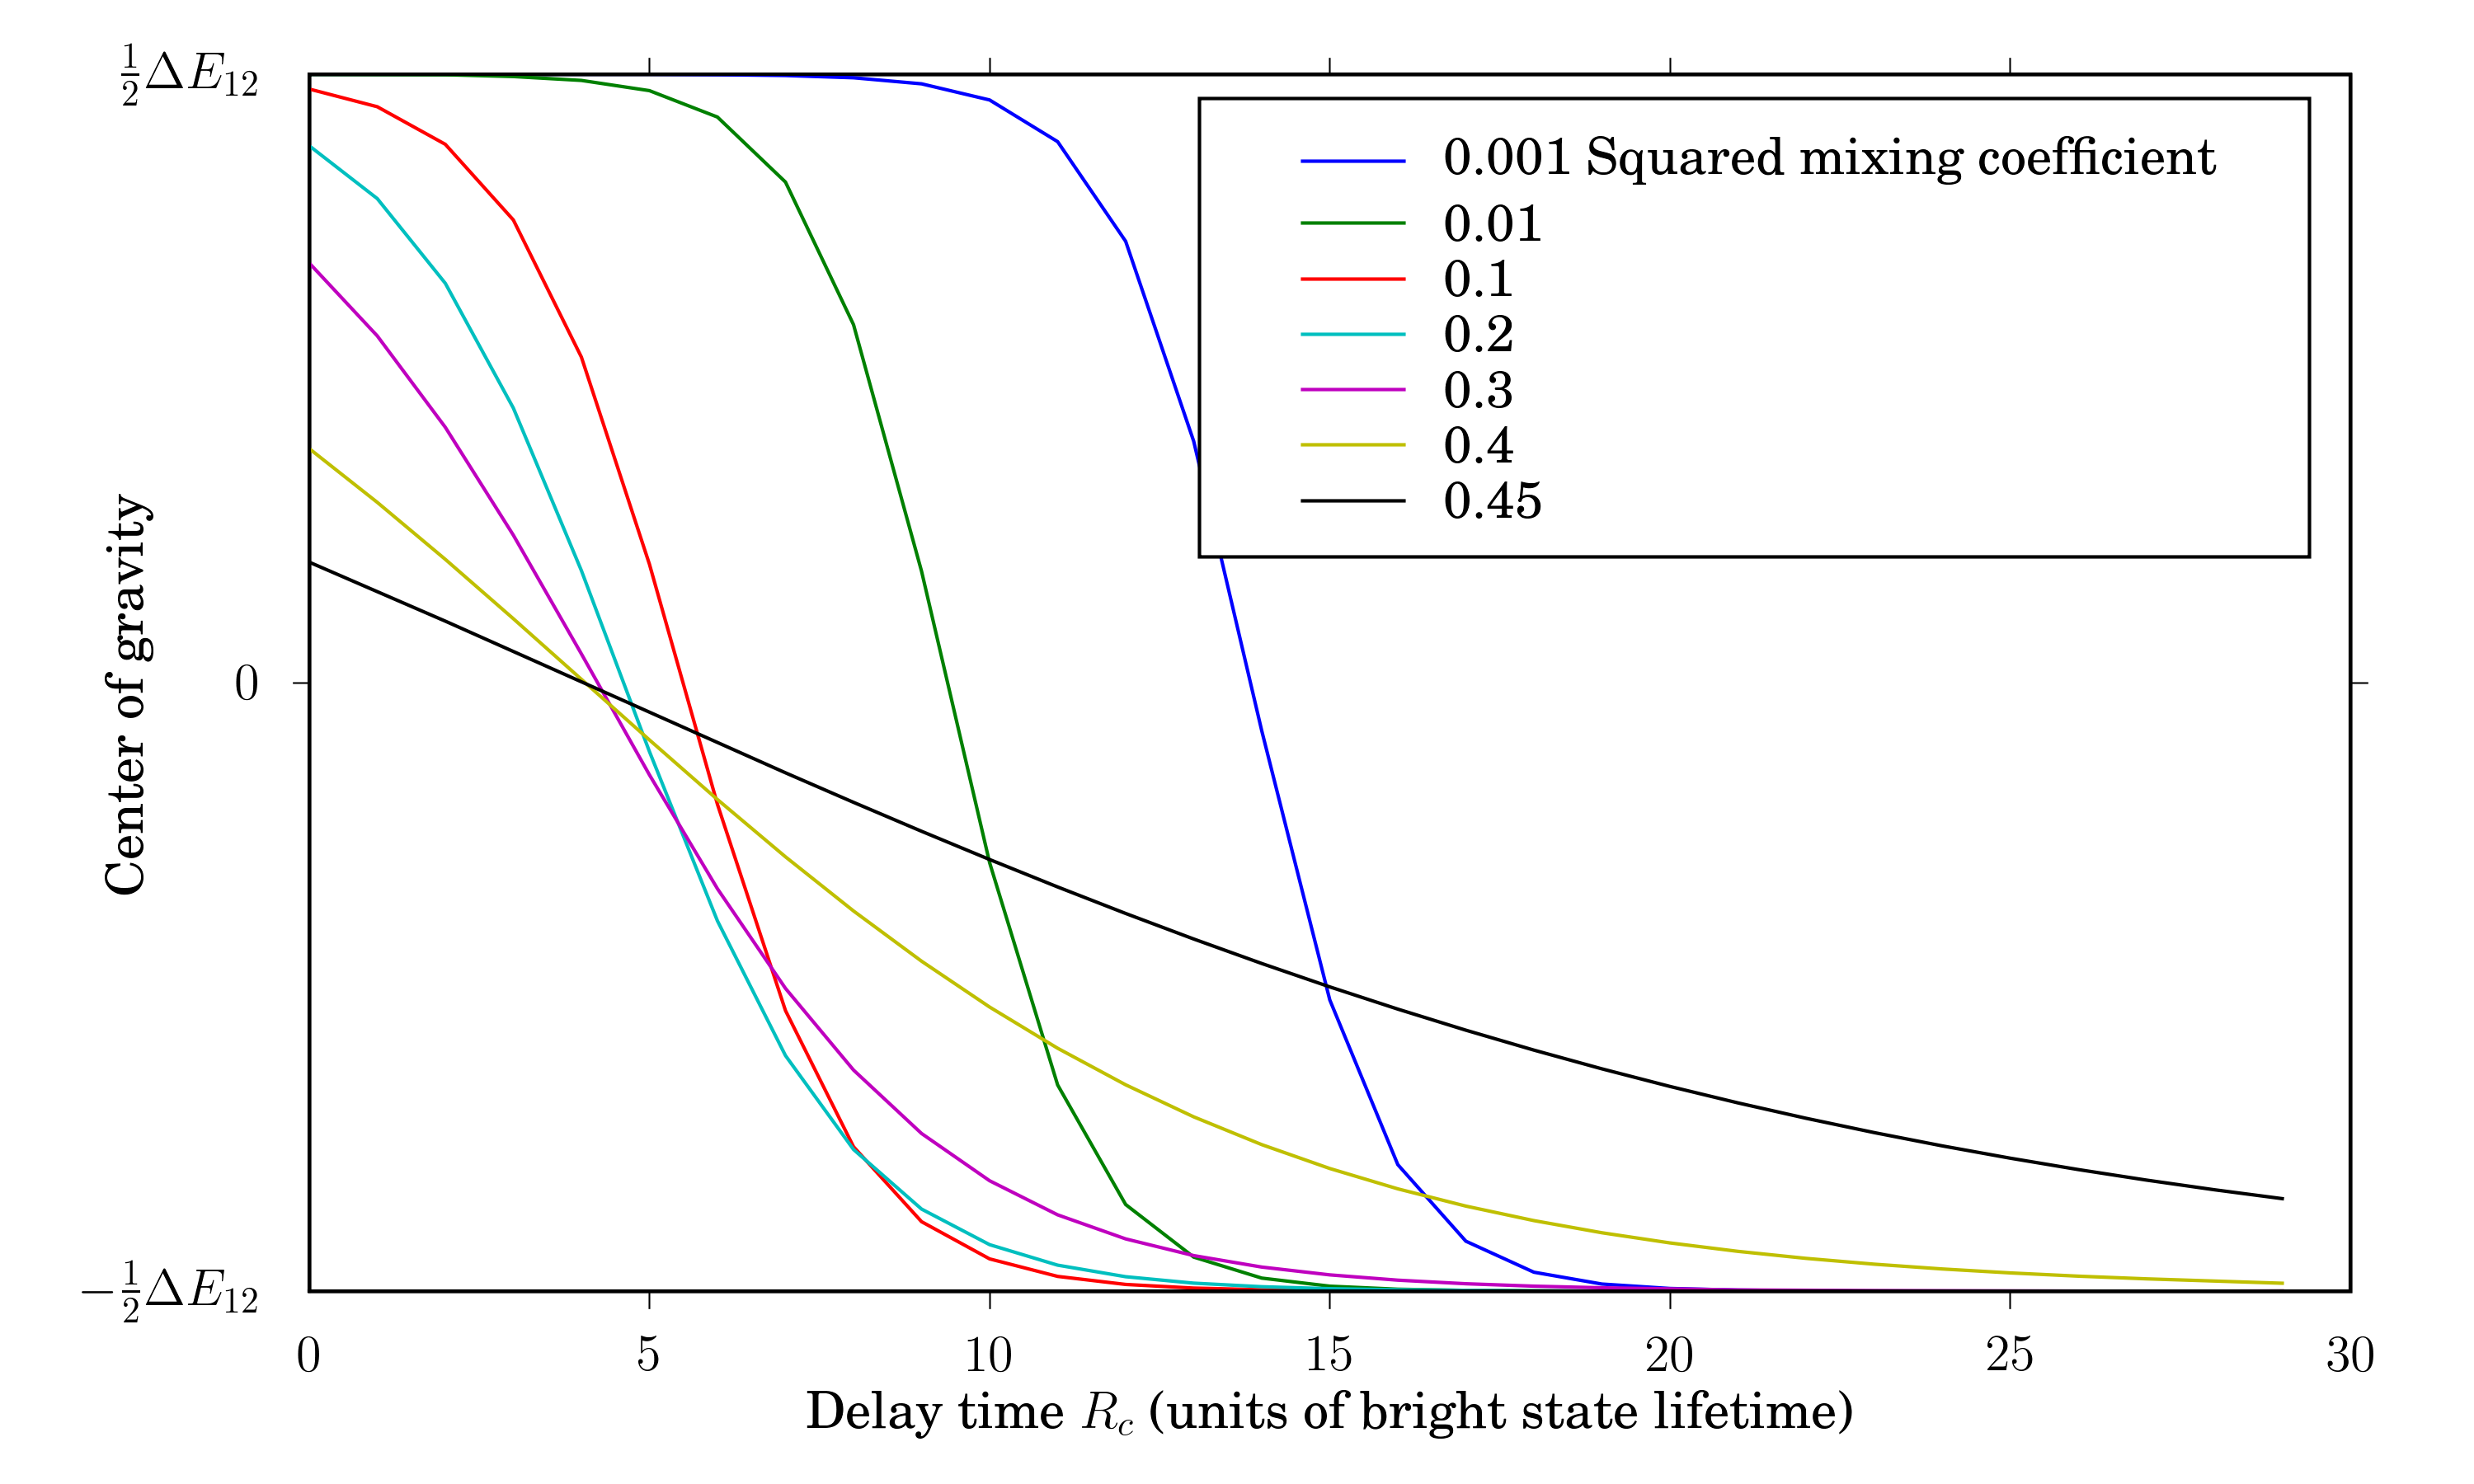
\includegraphics[width=6in]{cog-development.png}
\end{figure}

\subsection{Delayed fluorescence of a series of rotational
  transitions}

Information about the relative energy of a doorway level can be
recovered from the statistical properties of delayed fluorescence as a
function of rotational quantum number.  \POINT{Continue explaining the
general idea.}

\POINT{Present energy level spacings.} For a near-symmetric prolate
top in Hund's case ($b$), the spin-orbit selection rules are
\cite{stevens73}
\begin{equation}
  \begin{split}
    \Delta J &= 0 \\
    \Delta N &= 0, \pm 1\\
    \Delta K_a &= 0, \pm 1.
  \end{split}
\end{equation}
\TODO{Rewrite this.}  Due to the $\Delta N$ selection rule, a singlet
level $\ket{s;N=J}$ may interact with three rotational components of a
dark triplet state: $F_1$, $\ket{\ell;N=J-1}$; $F_2$,
$\ket{\ell;N=J}$; and $F_3$, $\ket{\ell;N=J+1}$.  The relative
energies of the three components are, in terms of the singlet
rotational quantum number $J$, \TODO{use different notation for
  $\Delta B$?}
\begin{equation}
  \label{eq:components}
  \Delta E_{s\ell}(J) = (E_{s} - E_{\ell}) +
  \begin{cases}
    \Delta B_{s\ell}J(J+1) + 2B_{\ell}J           
    & F_1 \text{ component}\\
    \Delta B_{s\ell}J(J+1)                      
    & F_2 \text{ component}\\
    \Delta B_{s\ell}J(J+1) - 2B_{\ell}J - 2B_{\ell} 
    & F_3 \text{ component}.\\
  \end{cases}
\end{equation}
In the approximation that $B_s \approx B_{\ell}$, the relative
energies of the $F_{1,2,3}$ components change linearly when plotted
against $J$.  The energy of the $F_2$ component relative to the
singlet state has a slope of approximately zero, while the $F_1$ and
$F_3$ components have slopes of approximately $\pm2B$.  The relative
energy differences between $S_1$ and $T(F_1,F_2,F_3)$ are plotted in
Figure \ref{fig:components}.

\begin{figure}
  \caption{\TODO{Change xlabel to $J$.}  Reduced term value plot of
    the three singlet$\sim$triplet roational components permitted by
    the spin-orbit operator in Hund's case ($b$).  The $F_1$ component
    corresponds to...  }
  \label{fig:components}
  \centering
  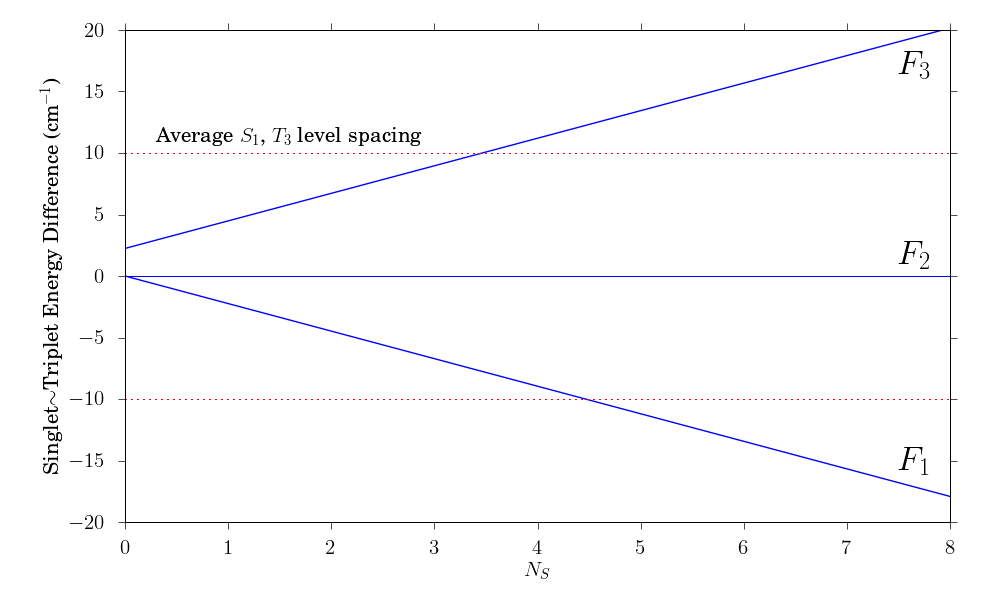
\includegraphics[width=6in]{f-components.png}
\end{figure}

Based on the existing assignment of a local $T_3$ perturber in $S_1$
$3 \nu_3$ $K_a$=1, as well as $T_3$ geometries prediced by \emph{ab
  initio} calculations, we expect the product $\Delta B_{s\ell}J(J+1)$
to remain small compared to $2BJ$ for any combination of $S_1$ and
$T_3$ vibrational levels \cite{mishra04, ventura03, thom07} up to the
maximum $J$ values ($J<8$) observed in our experiment .  \POINT{The
  figure is a good approximation to what we expect from the molecule.}

The total first-order spin-orbit matrix element between two
rovibrational states is given by the product of three factors: an
electronic spin-orbit matrix element, a vibrational overlap factor,
and a rotational factor arising from angular momentum coupling.  The
rotational factors are given for the general case of polyatomic
molecule asymmetric tops by Stevens and Brand \cite{stevens73}.  Plots
of the spin-orbit rotational factors are presented in Figure
\ref{fig:rotational-factors-0} for singlet levels with $K$=0, $K$=1
(Figure \ref{fig:rotational-factors-1}), and $K$=2 (Figure
\ref{fig:rotational-factors-2}).  With the exception of $\Delta N =
\Delta K = 0$ interactions, the rotational factors quickly approach
their asymptotic limits, usually between 0.1 and 0.6.  Even at low
values of $J$, the variation of rotational factor with rotational
quantum number is always less than a factor of 2.  \POINT{These
  variations are trumped by energy denominator and vibrational overlap
  effects.}

\begin{figure}
  \caption{Rotational factors for spin-orbit coupling in polyatomic
    molecules, $K_s$=0}
  \label{fig:rotational-factors-0}
  \centering
  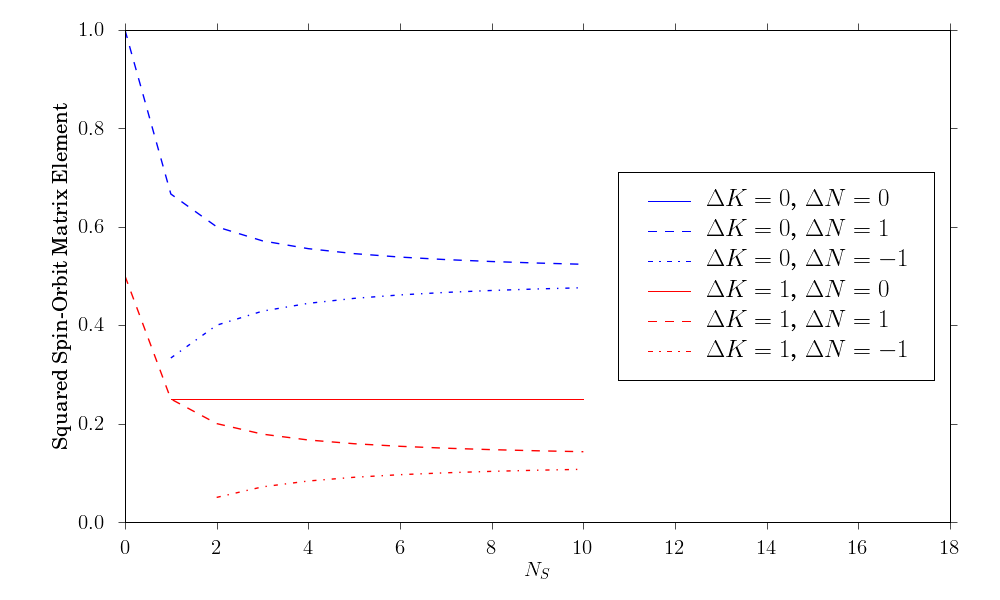
\includegraphics[width=6in]{rotational_factors_k0.png}
\end{figure}

\begin{figure}
  \caption{Rotational factors for spin-orbit coupling in polyatomic
    molecules, $K_s$=1}
  \label{fig:rotational-factors-1}
  \centering
  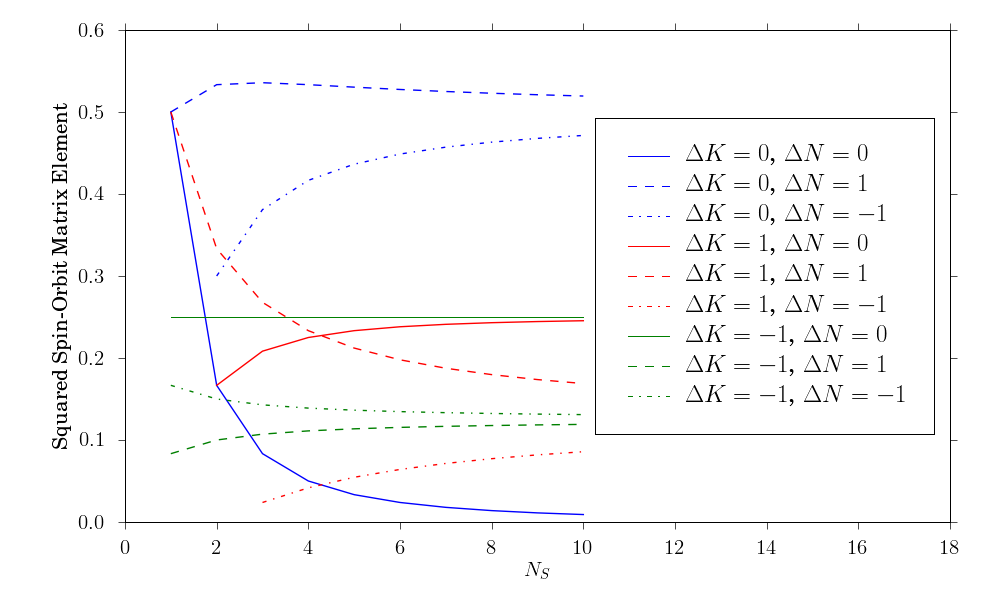
\includegraphics[width=6in]{rotational_factors_k1.png}
\end{figure}

\begin{figure}
  \caption{Rotational factors for spin-orbit coupling in polyatomic
    molecules, $K_s$=2}
  \label{fig:rotational-factors-2}
  \centering
  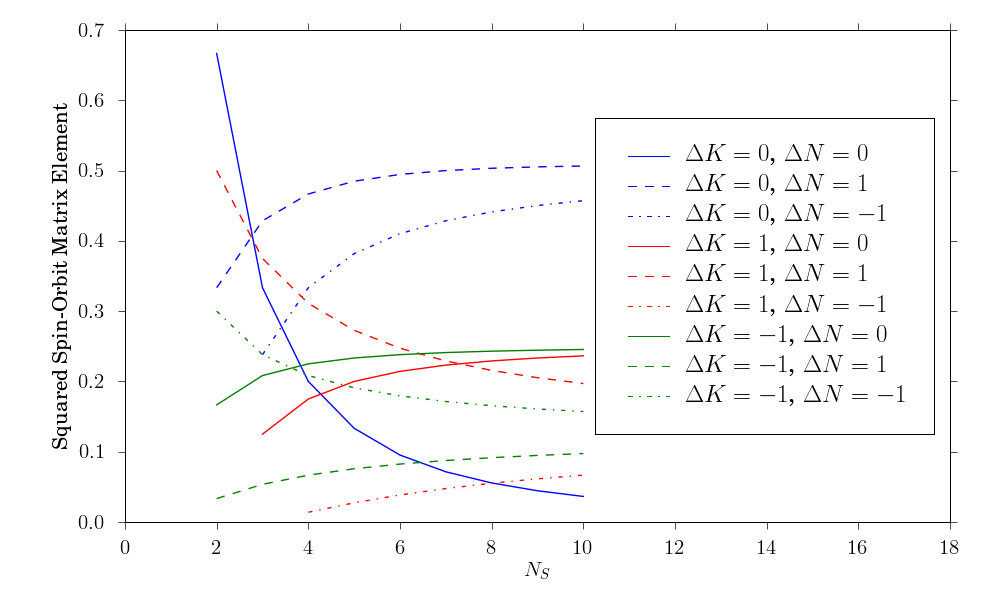
\includegraphics[width=6in]{rotational_factors_k2.png}
\end{figure}

\POINT{Expect vibrational factor to vary greatly.}  The effects of
widely varying vibrational overlap factors divide $S_1 \sim T_3$
perturbations into two classes: those where $H_{st}/\Delta E_{st} \ll
2B$, and those where $H_{st} / \Delta E_{st}$ is on the order of $2B$.

\POINT{Explain pattern when $H_{st}/\Delta E_{st} \ll 2B$.}
Perturbations in the first class, observable as a level shift, will
occur only once in the spectrum.  However, once a triplet level with
small vibrational overlap is found at a particular $J$, its energy
above or below the perturbed singlet level may be found according to
Equation \ref{eq:components}.

\POINT{Explain pattern when $H_{st}/\Delta E_{st} \approx 2B$.}
Perturbations falling into the second class will affect the
singlet$\sim$triplet coupling at several values of $J$; these are the
distant $T_3$ doorways with which we are most concerned.  \TODO{Plot
  mixing coefficients of distant doorways as a fcn of rotational
  quantum number.  Trend will be: weakly coupled states turn on/off
  suddenly, strongly coupled states are visible for several values of
  $N$.}

\section{Experiment}

\TODO{Adapt this from paper.}  SEELEM is a versatile and sensitive
technique for investigating molecules in ``dark'' (weakly-fluorescing)
metastable states populated by laser excitation.1-6 In the SEELEM
experiment, a molecular beam of acetylene is excited by a $\sim$5 ns
FWHM pulsed tunable laser into spin-rotation-vibration eigenstates of
metastable electronic states via weak, nominally forbidden
transitions. After excitation, the long-lived species must travel 35
cm before colliding with an Au metal detector surface, where an
electron is ejected in a de-excitation process. Two criteria must be
met for electron ejection by a metastable species. First, the vertical
electronic energy of the metastable approaching the surface must
exceed the work function of the metal ($\Phi_{\text{Au}}$ = 5.1
eV). Second, the radiative lifetime of the detected metastable
eigenstate ($\tau_\text{rad}$) must exceed the flight time from the
point of laser excitation to the SEELEM surface ($\Delta$t=300
$\mu$s).

A sample of acetylene (BOC gases) at a backing pressure of one
atmosphere was pulsed through a 0.5 mm diameter nozzle operating at 10
Hz into a diffusion pumped vacuum chamber at $\sim$5\e{-5} torr.  An
Nd:YAG pumped, frequency-doubled dye laser (220 nm) excited the
acetylene molecules in the pulsed jet expansion 2 cm downstream from
the nozzle orifice. UV-LIF was detected perpendicular to the plane
defined by the intersection of the pulsed molecular and laser beams
using f/1.2 collection optics, a fluorescence filter (UG-11) to reduce
scattered laser light, and a PMT (Hamamatsu model R375). The
fluorescence signal was averaged by a boxcar integrator and
recorded. For SEELEM detection, the excited molecules in the pulsed
expansion passed through a conical skimmer (3mm diameter) to form a
collimated molecular beam, which traveled into a differentially pumped
detector chamber maintained at $\sim$4\e{-7} torr, and collided with a
heated (300\degrees\ C) Au metal surface 35 cm downstream from the
point of laser excitation. The SEELEM detector was identical to that
used in the previously described apparatus with Au foil ($\Phi$ = 5.1
eV) as the detector surface.  Particle counting techniques, including
a multichannel scalar (Oxford Tennelec Nucleus Inc. MCS-II v2.091)
were used to record laser-excited metastable counts as a function of
laser frequency, along with the simultaneously recorded LIF
spectra. Both SEELEM and LIF signals were averaged over 100 laser
shots per data point.  The typical signal level for SEELEM detection
of acetylene was 2-20 counts per laser pulse.

\section{LIF/SEELEM intensity distributions}

\subsection{The $2^23^1$ $K_a$=1 sublevel}

\POINT{SEELEM spectrum of $2^2 3^1$ (Oct/Nov 2006, see ``similitude''
  calculations, p.62 of Sep 2006--Jan 2007 notebook.)}  This spectrum
is shown in Figure \ref{fig:spectrum-2231}.  For this band, several
scans were repeated with finer frequency steps.  Figure
\ref{fig:spectrum-2231-q123} shows the first three transitions of the
Q-branch.  Figure \ref{fig:spectrum-2231-q1r0} shows the two
transitions, Q(1) and R(0).  These two transitions have the same upper
state rotational quantum number ($J'=1$), but differ in parity (having
$f$- and $e$-symmetry, respectively).
% Selection rules: Q   -> e-f
%                  P,R -> e-e, f-f

\begin{figure}
  \caption{
    % Simultaneously recorded LIF and SEELEM spectra of the
    % acetylene $V^2_04^2_0K^1_0$ $\tilde{A}^1A_u \leftarrow
    % \tilde{X}^1\Sigma_g$ transition.
    Simultaneously recorded surface electron ejection by laser excited
    metastables (SEELEM, upper trace) and ultraviolet laser-induced
    fluorescence (UV-LIF, lower trace) spectra of the $2^23^1$ $K_a$=1
    sublevel of the $\tilde{A}^1A_u \leftarrow \tilde{X} ^1\Sigma_g^+$
    electronic transition. A delayed, integrated fluorescence signal
    is shown as a dotted trace in the UV-LIF spectrum.}
  \label{fig:spectrum-2231}
  \centering
  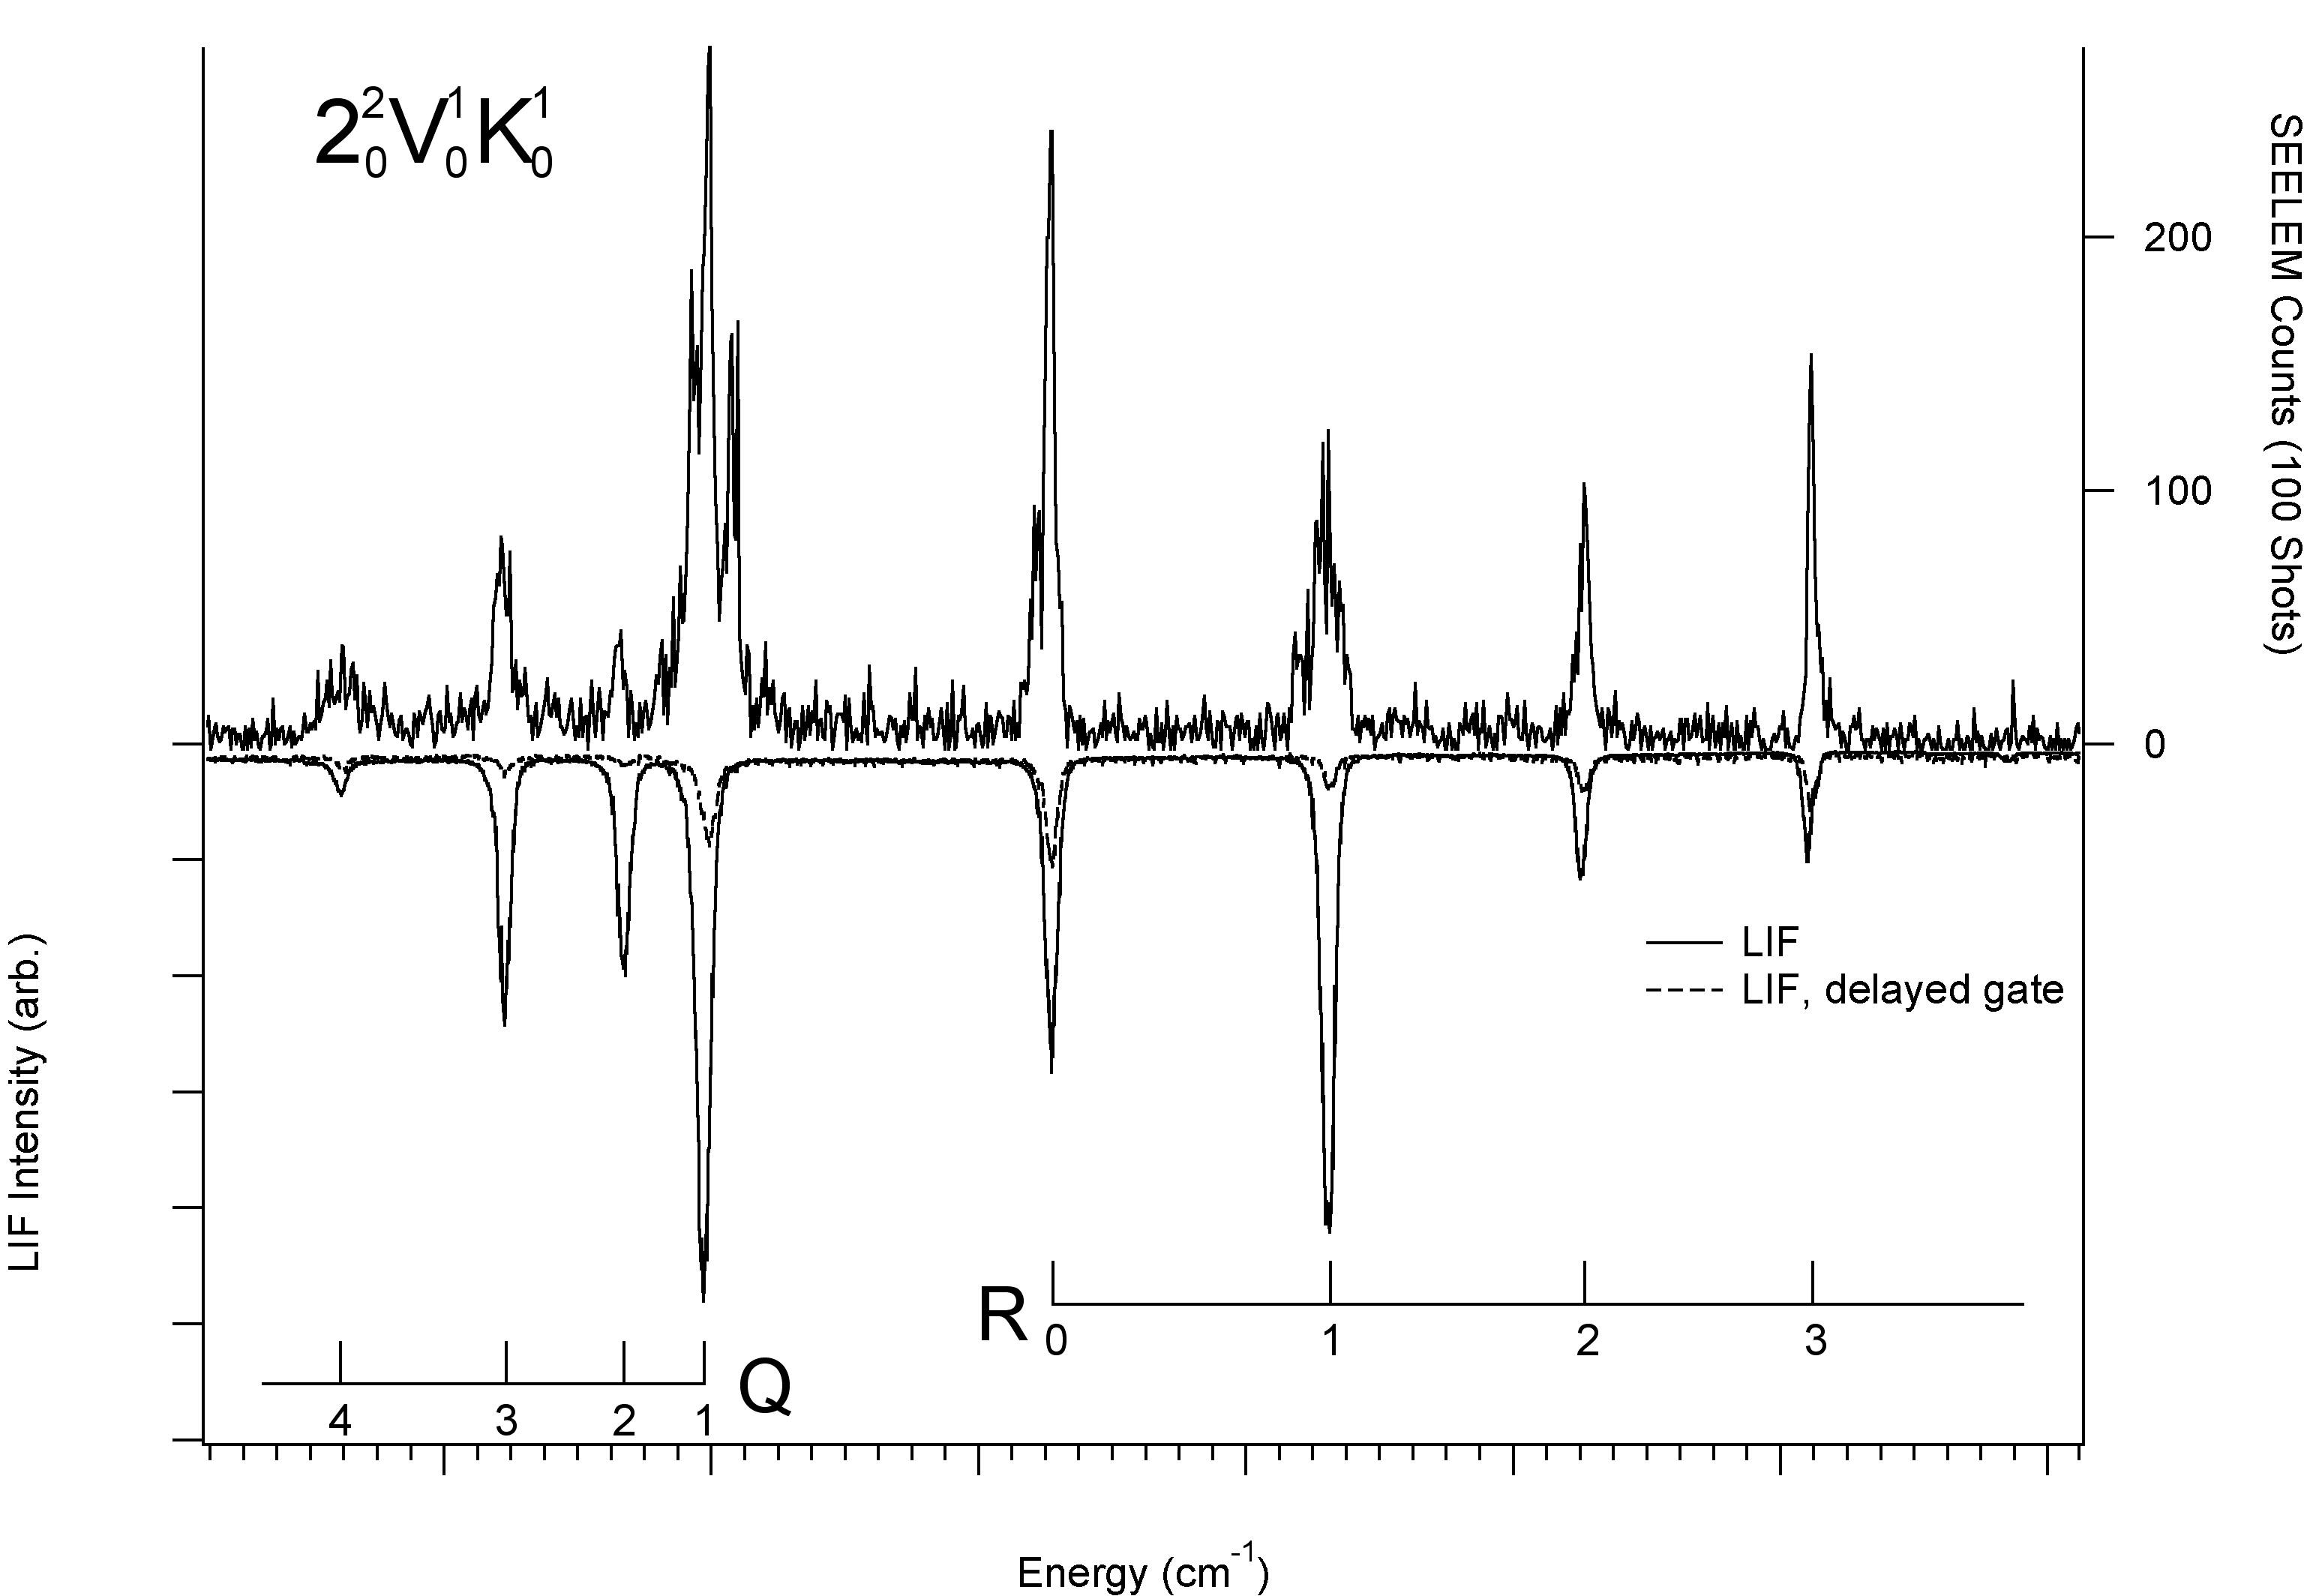
\includegraphics[width=8in,angle=90]{spectrum-2231.png}
\end{figure}

\begin{figure}
  \caption{
    % Simultaneously recorded LIF and SEELEM spectra of the
    % acetylene $V^2_04^2_0K^1_0$ $\tilde{A}^1A_u \leftarrow
    % \tilde{X}^1\Sigma_g$ transition.
    Simultaneously recorded surface electron ejection by laser excited
    metastables (SEELEM, upper trace) and ultraviolet laser-induced
    fluorescence (UV-LIF, lower trace) spectra of the $2^23^1$ $K_a$=1
    sublevel of the $\tilde{A}^1A_u \leftarrow \tilde{X} ^1\Sigma_g^+$
    electronic transition. A delayed, integrated fluorescence signal
    is shown as a dotted trace in the UV-LIF spectrum.}
  \label{fig:spectrum-2231-q123}
  \centering
  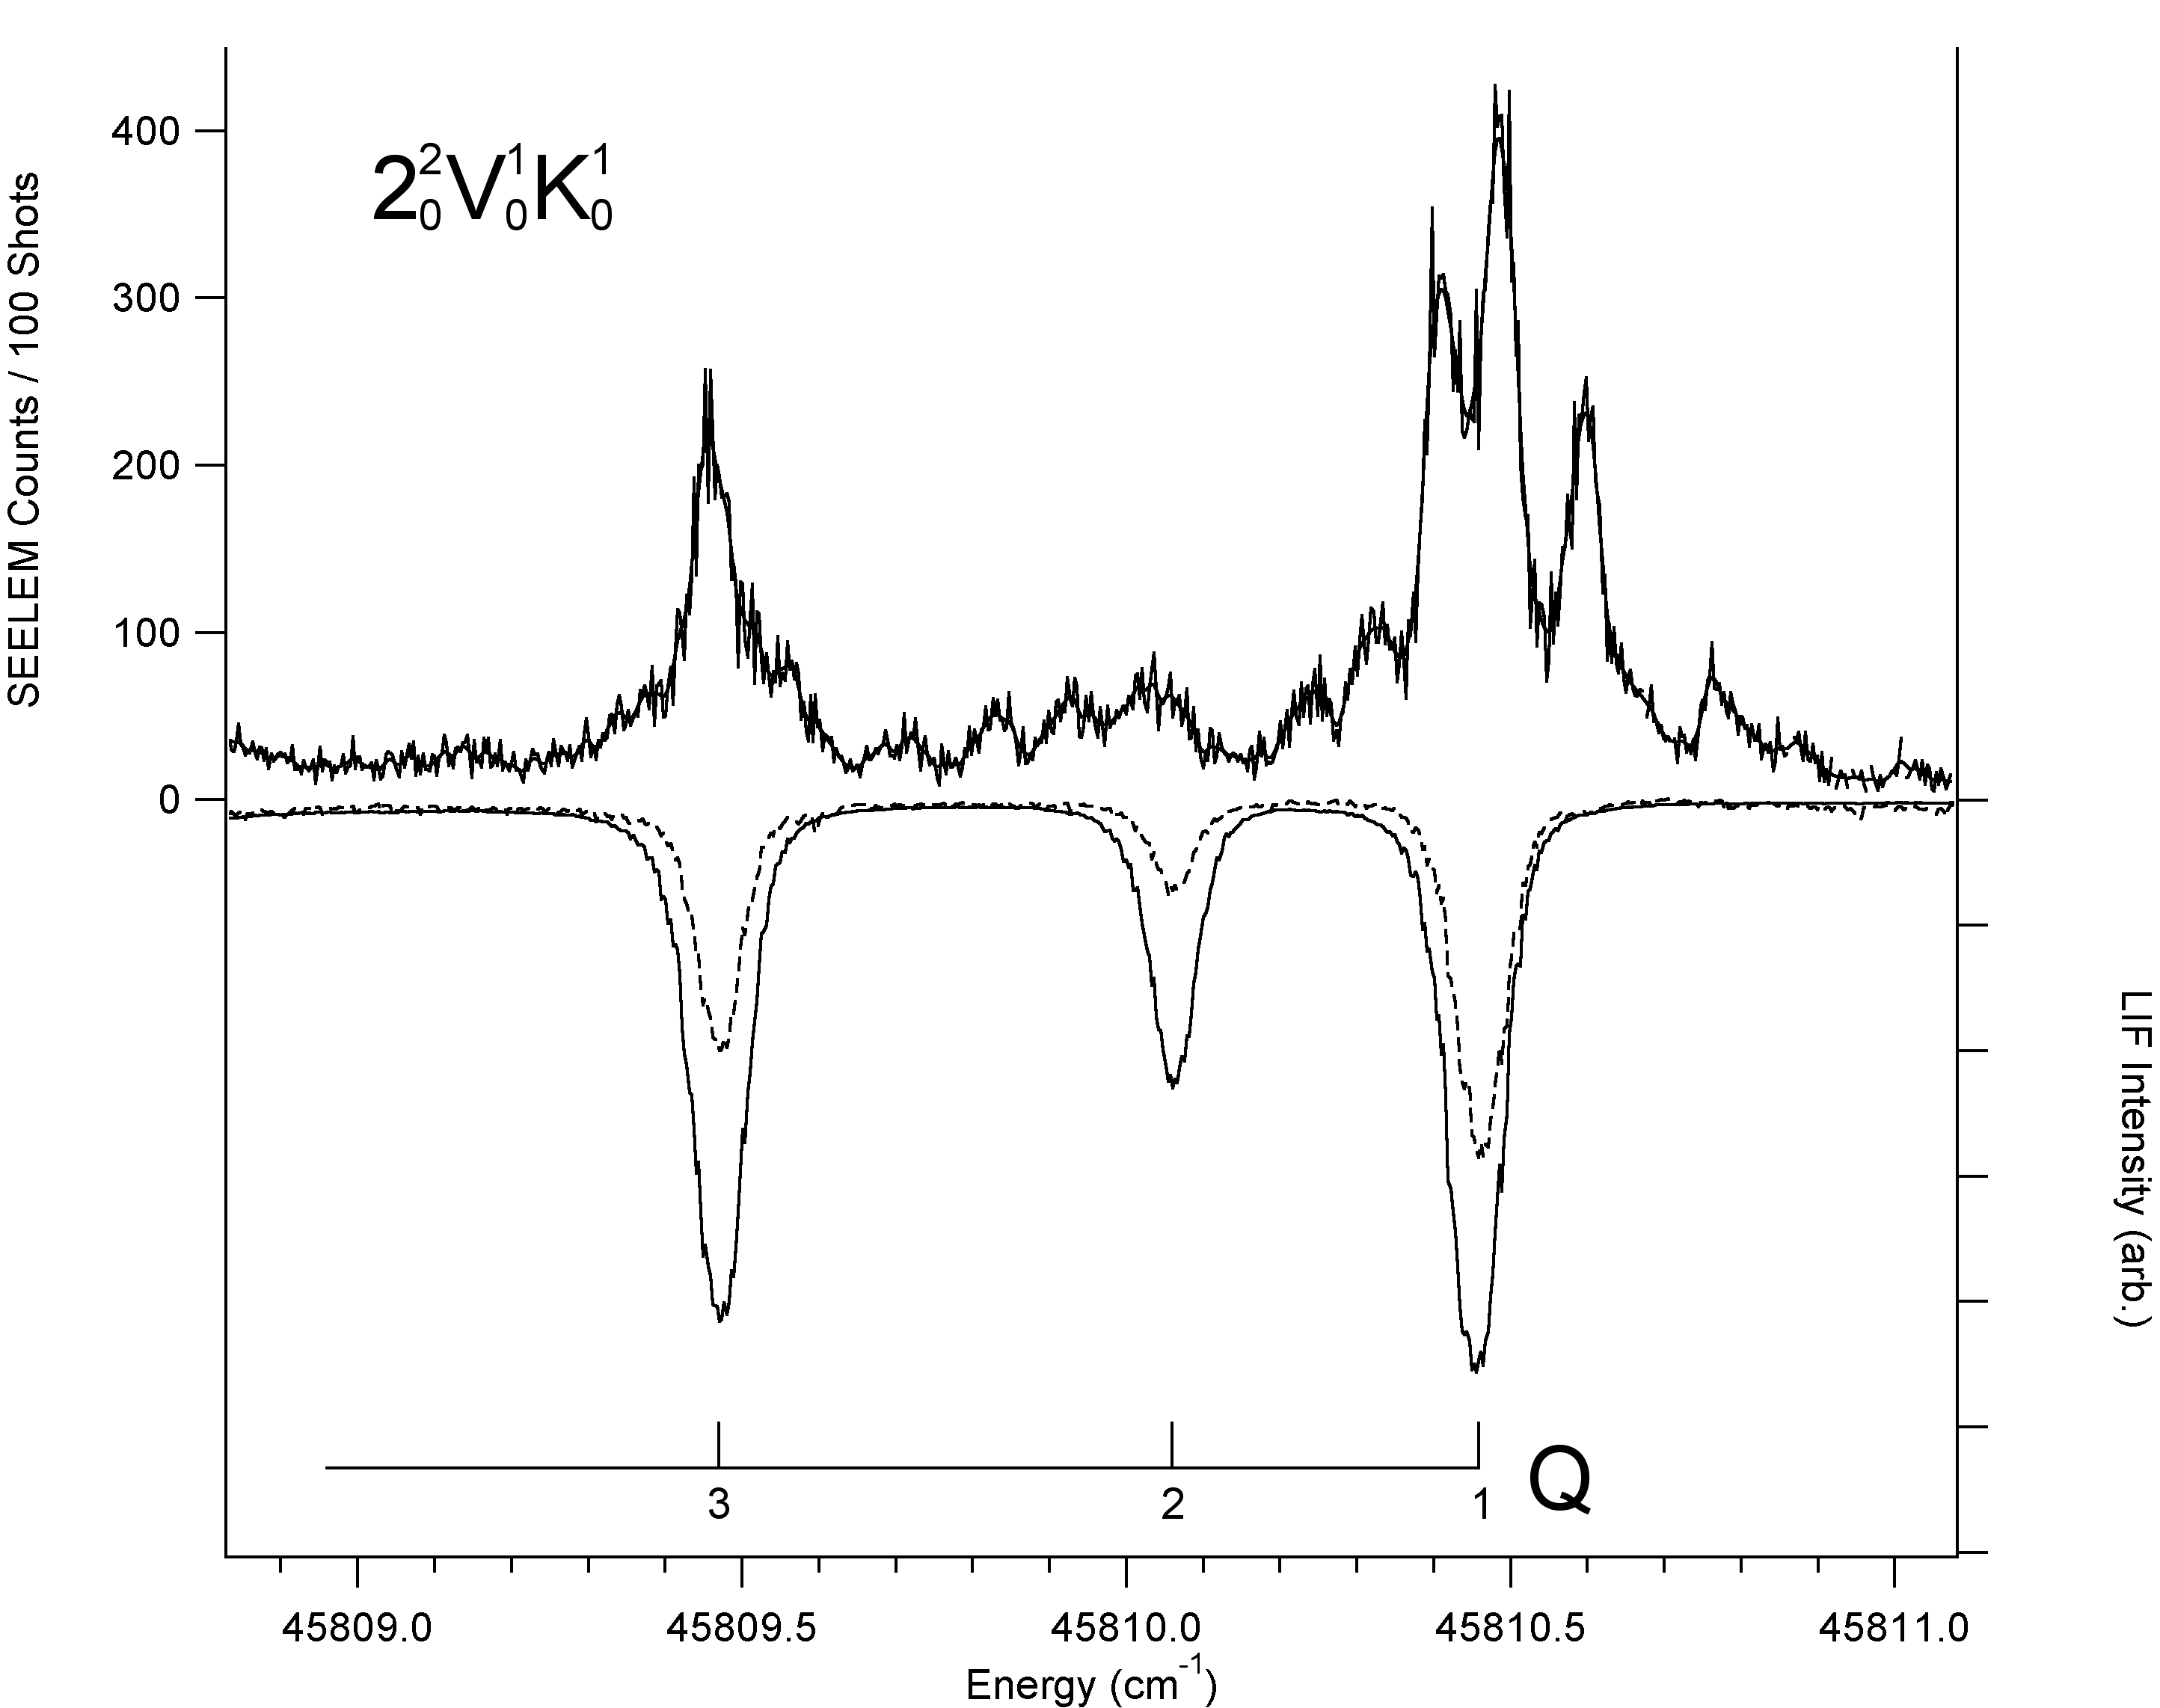
\includegraphics[width=6in]{spectrum-2231-Q123.png}
\end{figure}

\begin{figure}
  \caption{
    % Simultaneously recorded LIF and SEELEM spectra of the
    % acetylene $V^2_04^2_0K^1_0$ $\tilde{A}^1A_u \leftarrow
    % \tilde{X}^1\Sigma_g$ transition.
    Simultaneously recorded surface electron ejection by laser excited
    metastables (SEELEM, upper trace) and ultraviolet laser-induced
    fluorescence (UV-LIF, lower trace) spectra of the $2^23^1$ $K_a$=1
    sublevel of the $\tilde{A}^1A_u \leftarrow \tilde{X} ^1\Sigma_g^+$
    electronic transition. A delayed, integrated fluorescence signal
    is shown as a dotted trace in the UV-LIF spectrum.}
  \label{fig:spectrum-2231-q1r0}
  \centering
  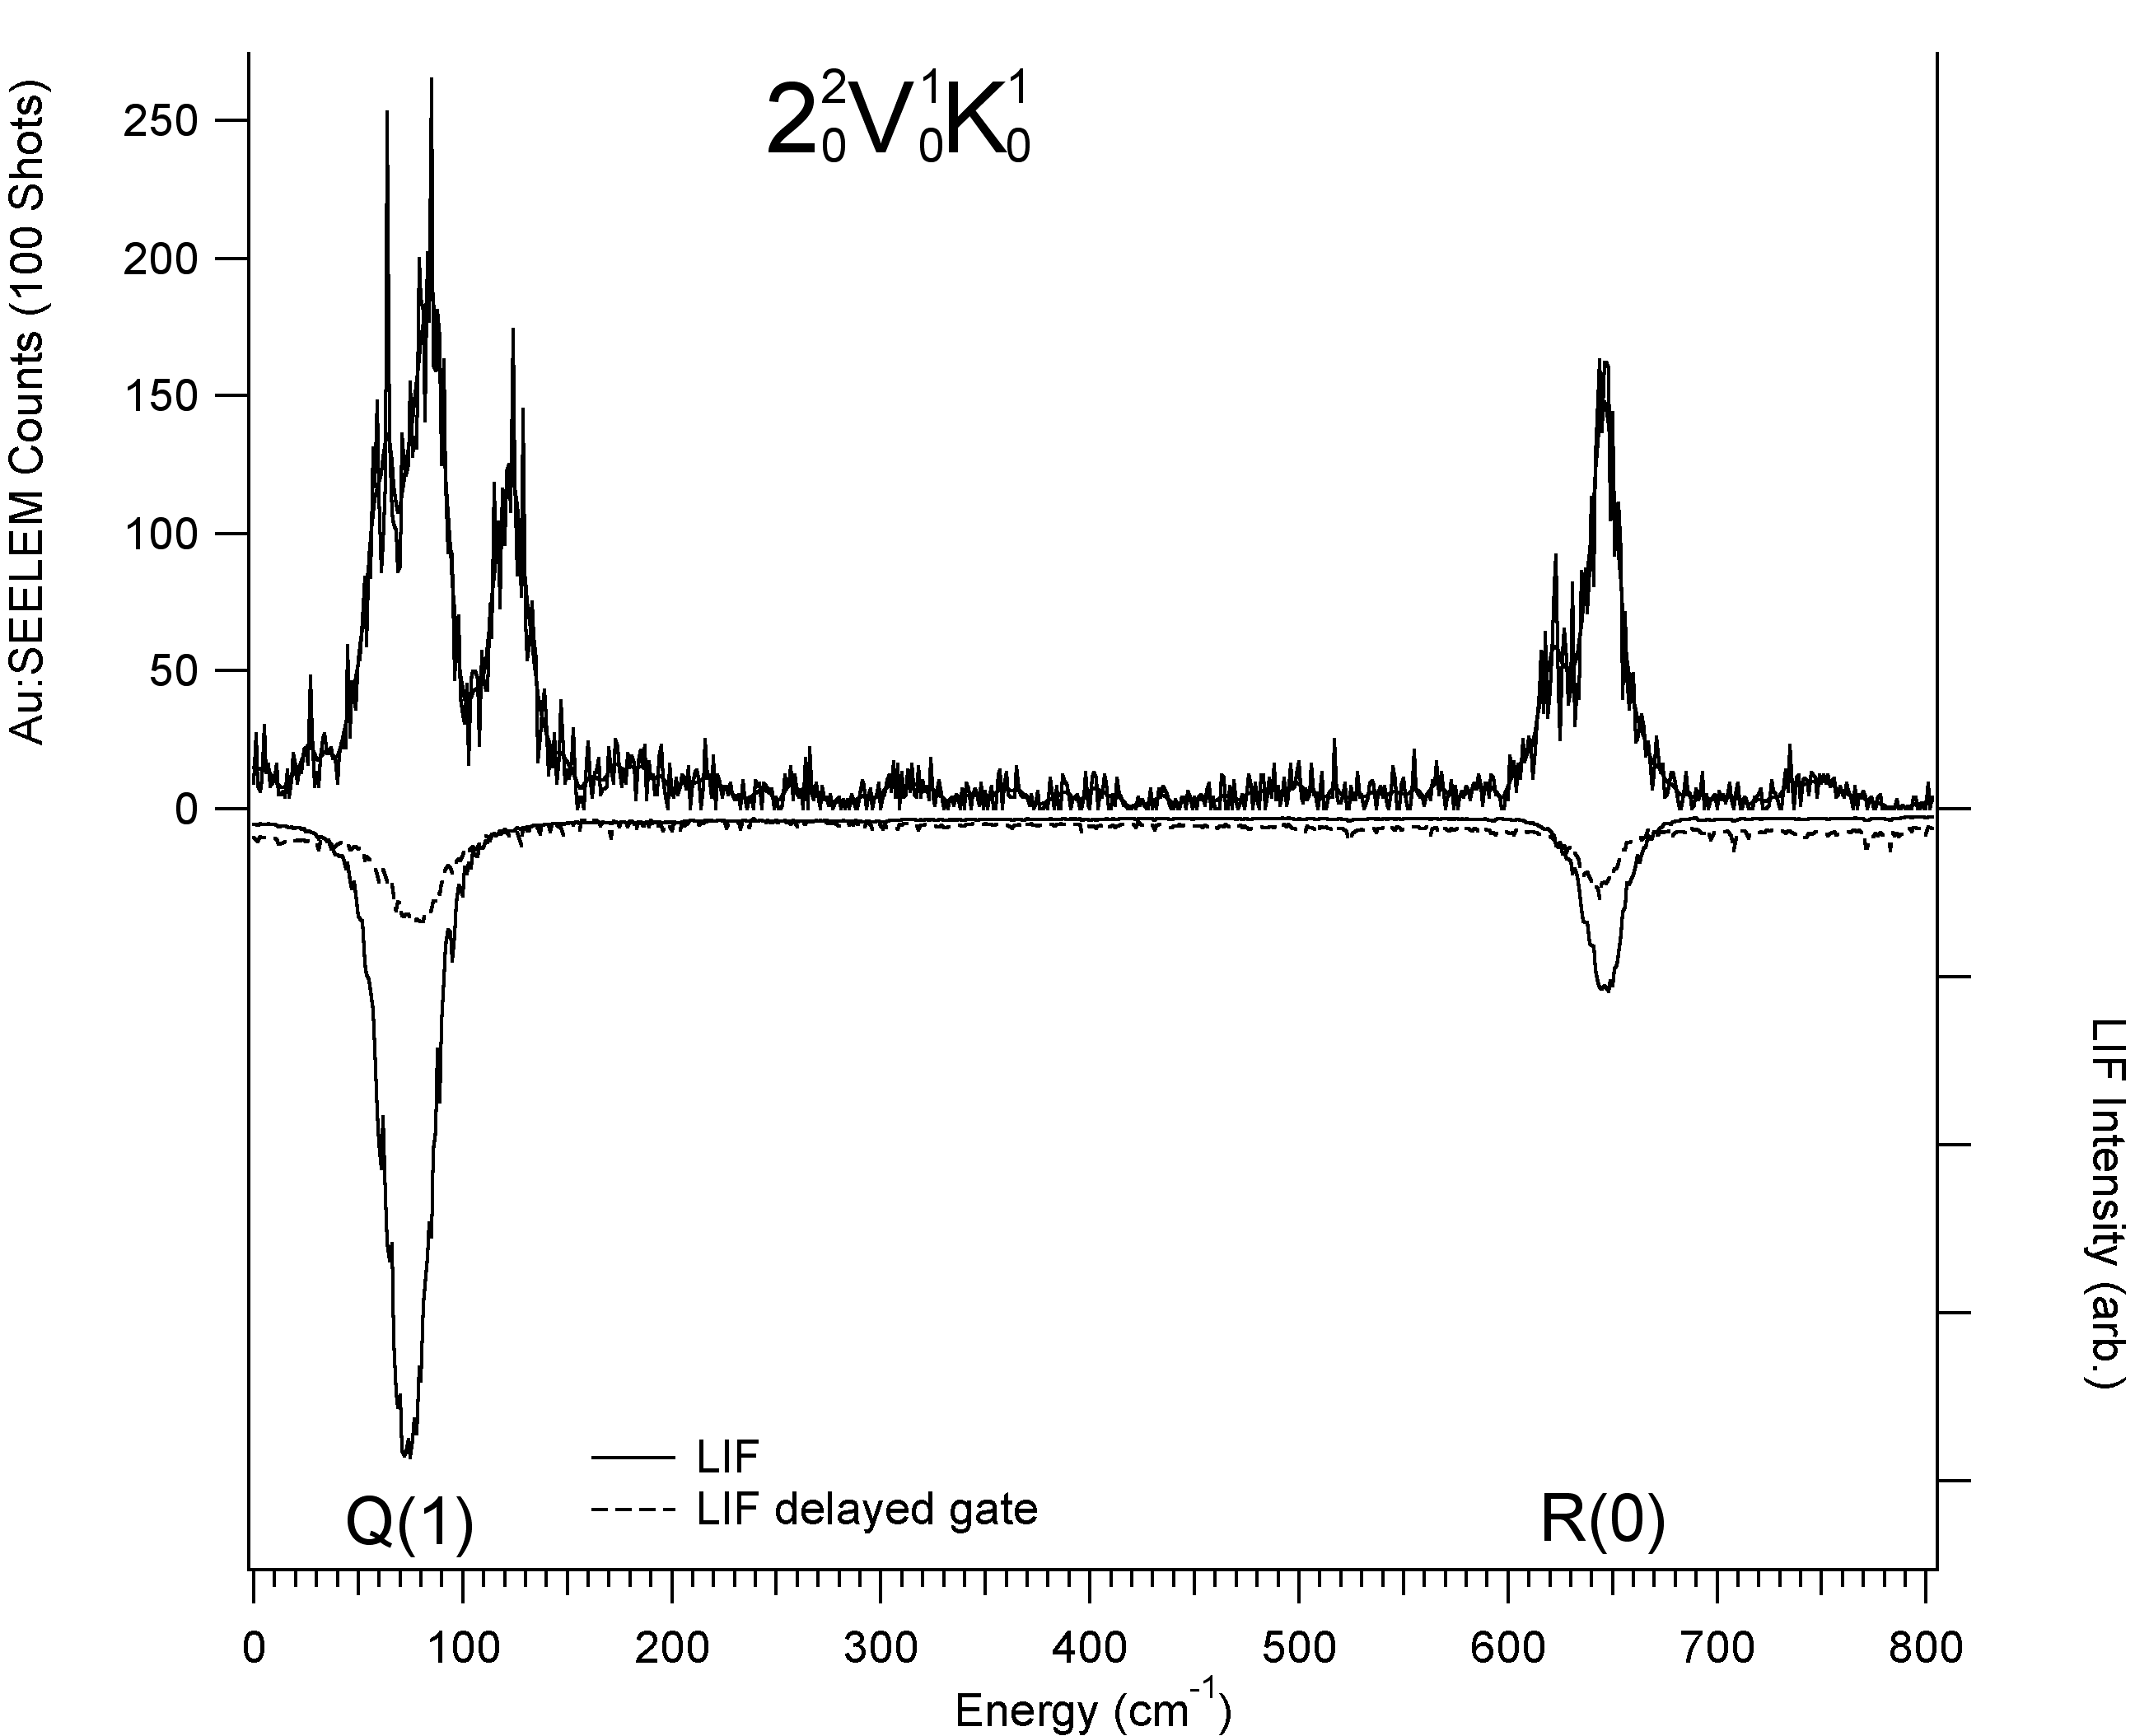
\includegraphics[width=6in]{spectrum-2231-Q1R0.png}
\end{figure}

\TODO{Get trace data from MIT.}

\subsection{The $2^13^2$ $K_a$=1 sublevel}

\POINT{SEELEM spectrum of $2^1 3^2$ P, Q-branch (See Jan 16A+B,
  p.124--127 of 9/2006--1/2007 notebook, also assignments on p.2 of
  1/2007--3/2007 notebook.)}  This spectrum is shown in Figure
\ref{fig:spectrum-2132}.

\begin{figure}
  \caption{
    % Simultaneously recorded LIF and SEELEM spectra of the
    % acetylene $V^2_04^2_0K^1_0$ $\tilde{A}^1A_u \leftarrow
    % \tilde{X}^1\Sigma_g$ transition.
    Simultaneously recorded surface electron ejection by laser excited
    metastables (SEELEM, upper trace) and ultraviolet laser-induced
    fluorescence (UV-LIF, lower trace) spectra of the $2^13^2$ $K_a$=1
    sublevel of the $\tilde{A}^1A_u \leftarrow \tilde{X} ^1\Sigma_g^+$
    electronic transition. A delayed, integrated fluorescence signal
    is shown as a dotted trace in the UV-LIF spectrum.}
  \label{fig:spectrum-2132}
  \centering
  \includegraphics[width=8in,angle=90]{spectrum-2132.pdf}
\end{figure}

\TODO{Import calibration points from IGOR.}

Figure \ref{fig:2132-qbranch-cog-delay} shows the shifting center of
gravity of a series of rotational lines Q(1-5) in the LIF spectrum of
the $2^13^2$ $K_a$=1 sublevel.

\begin{figure}
  \caption{Shifting center of gravity of a series of rotational lines
    Q(1-5) in the LIF spectrum of the $2^13^2$ $K_a$=1 sublevel.}
  \label{fig:2132-qbranch-cog-delay}
  \centering
  \includegraphics[width=6in]{2132-qbranch-cog-delay.pdf}
\end{figure}

Figure \ref{fig:2132-indiv-cog-delay} shows the shifting center of
gravity of individual transitions Q(1-5) in the LIF spectrum of
the $2^13^2$ $K_a$=1 sublevel.

\begin{figure}
  \caption{Shifting center of gravity of a series of individual
    transitions Q(1-5) in the LIF spectrum of the $2^13^2$ $K_a$=1
    sublevel.}
  \label{fig:2132-indiv-cog-delay}
  \centering
  \includegraphics[width=6in]{2132-indiv-cog-delay.pdf}
\end{figure}

Figure \ref{fig:2132-indiv-var-delay} shows the increasing variance of
individual transitions Q(1-5) in the LIF spectrum of the $2^13^2$
$K_a$=1 sublevel.  \POINT{Huge difference between $J'=1,2$ and
  $J'=3,4,5$ is consistent with coupling to an energetically distant
  doorway with $K_a$=2 via the $F_1$ component.}

\begin{figure}
  \caption{Spectral variance plotted as a function of LIF delay time
    for a series of individual transitions Q(1-5) in the LIF spectrum
    of the $2^13^2$ $K_a$=1 sublevel.}
  \label{fig:2132-indiv-var-delay}
  \centering
  \includegraphics[width=6in]{2132-indiv-var-delay.pdf}
\end{figure}

\subsection{The $3^3$ $K_a$=2 sublevel}

\POINT{SEELEM spectrum of $3^3$ $K=2$ hot band (See Jan 22C, p.31,34
  of 1/2007--3/2007 notebook.)}  This spectrum is shown in Figure
\ref{fig:spectrum-33k2}.

\begin{figure}
  \caption{
    Simultaneously recorded surface electron ejection by laser excited
    metastables (SEELEM, upper trace) and ultraviolet laser-induced
    fluorescence (UV-LIF, lower trace) spectra of the $3^3$ $K_a$=2
    sublevel of the $\tilde{A}^1A_u \leftarrow \tilde{X} ^1\Sigma_g^+$
    electronic transition. A delayed, integrated fluorescence signal
    is shown as a dotted trace in the UV-LIF spectrum.}
  \label{fig:spectrum-33k2}
  \centering
  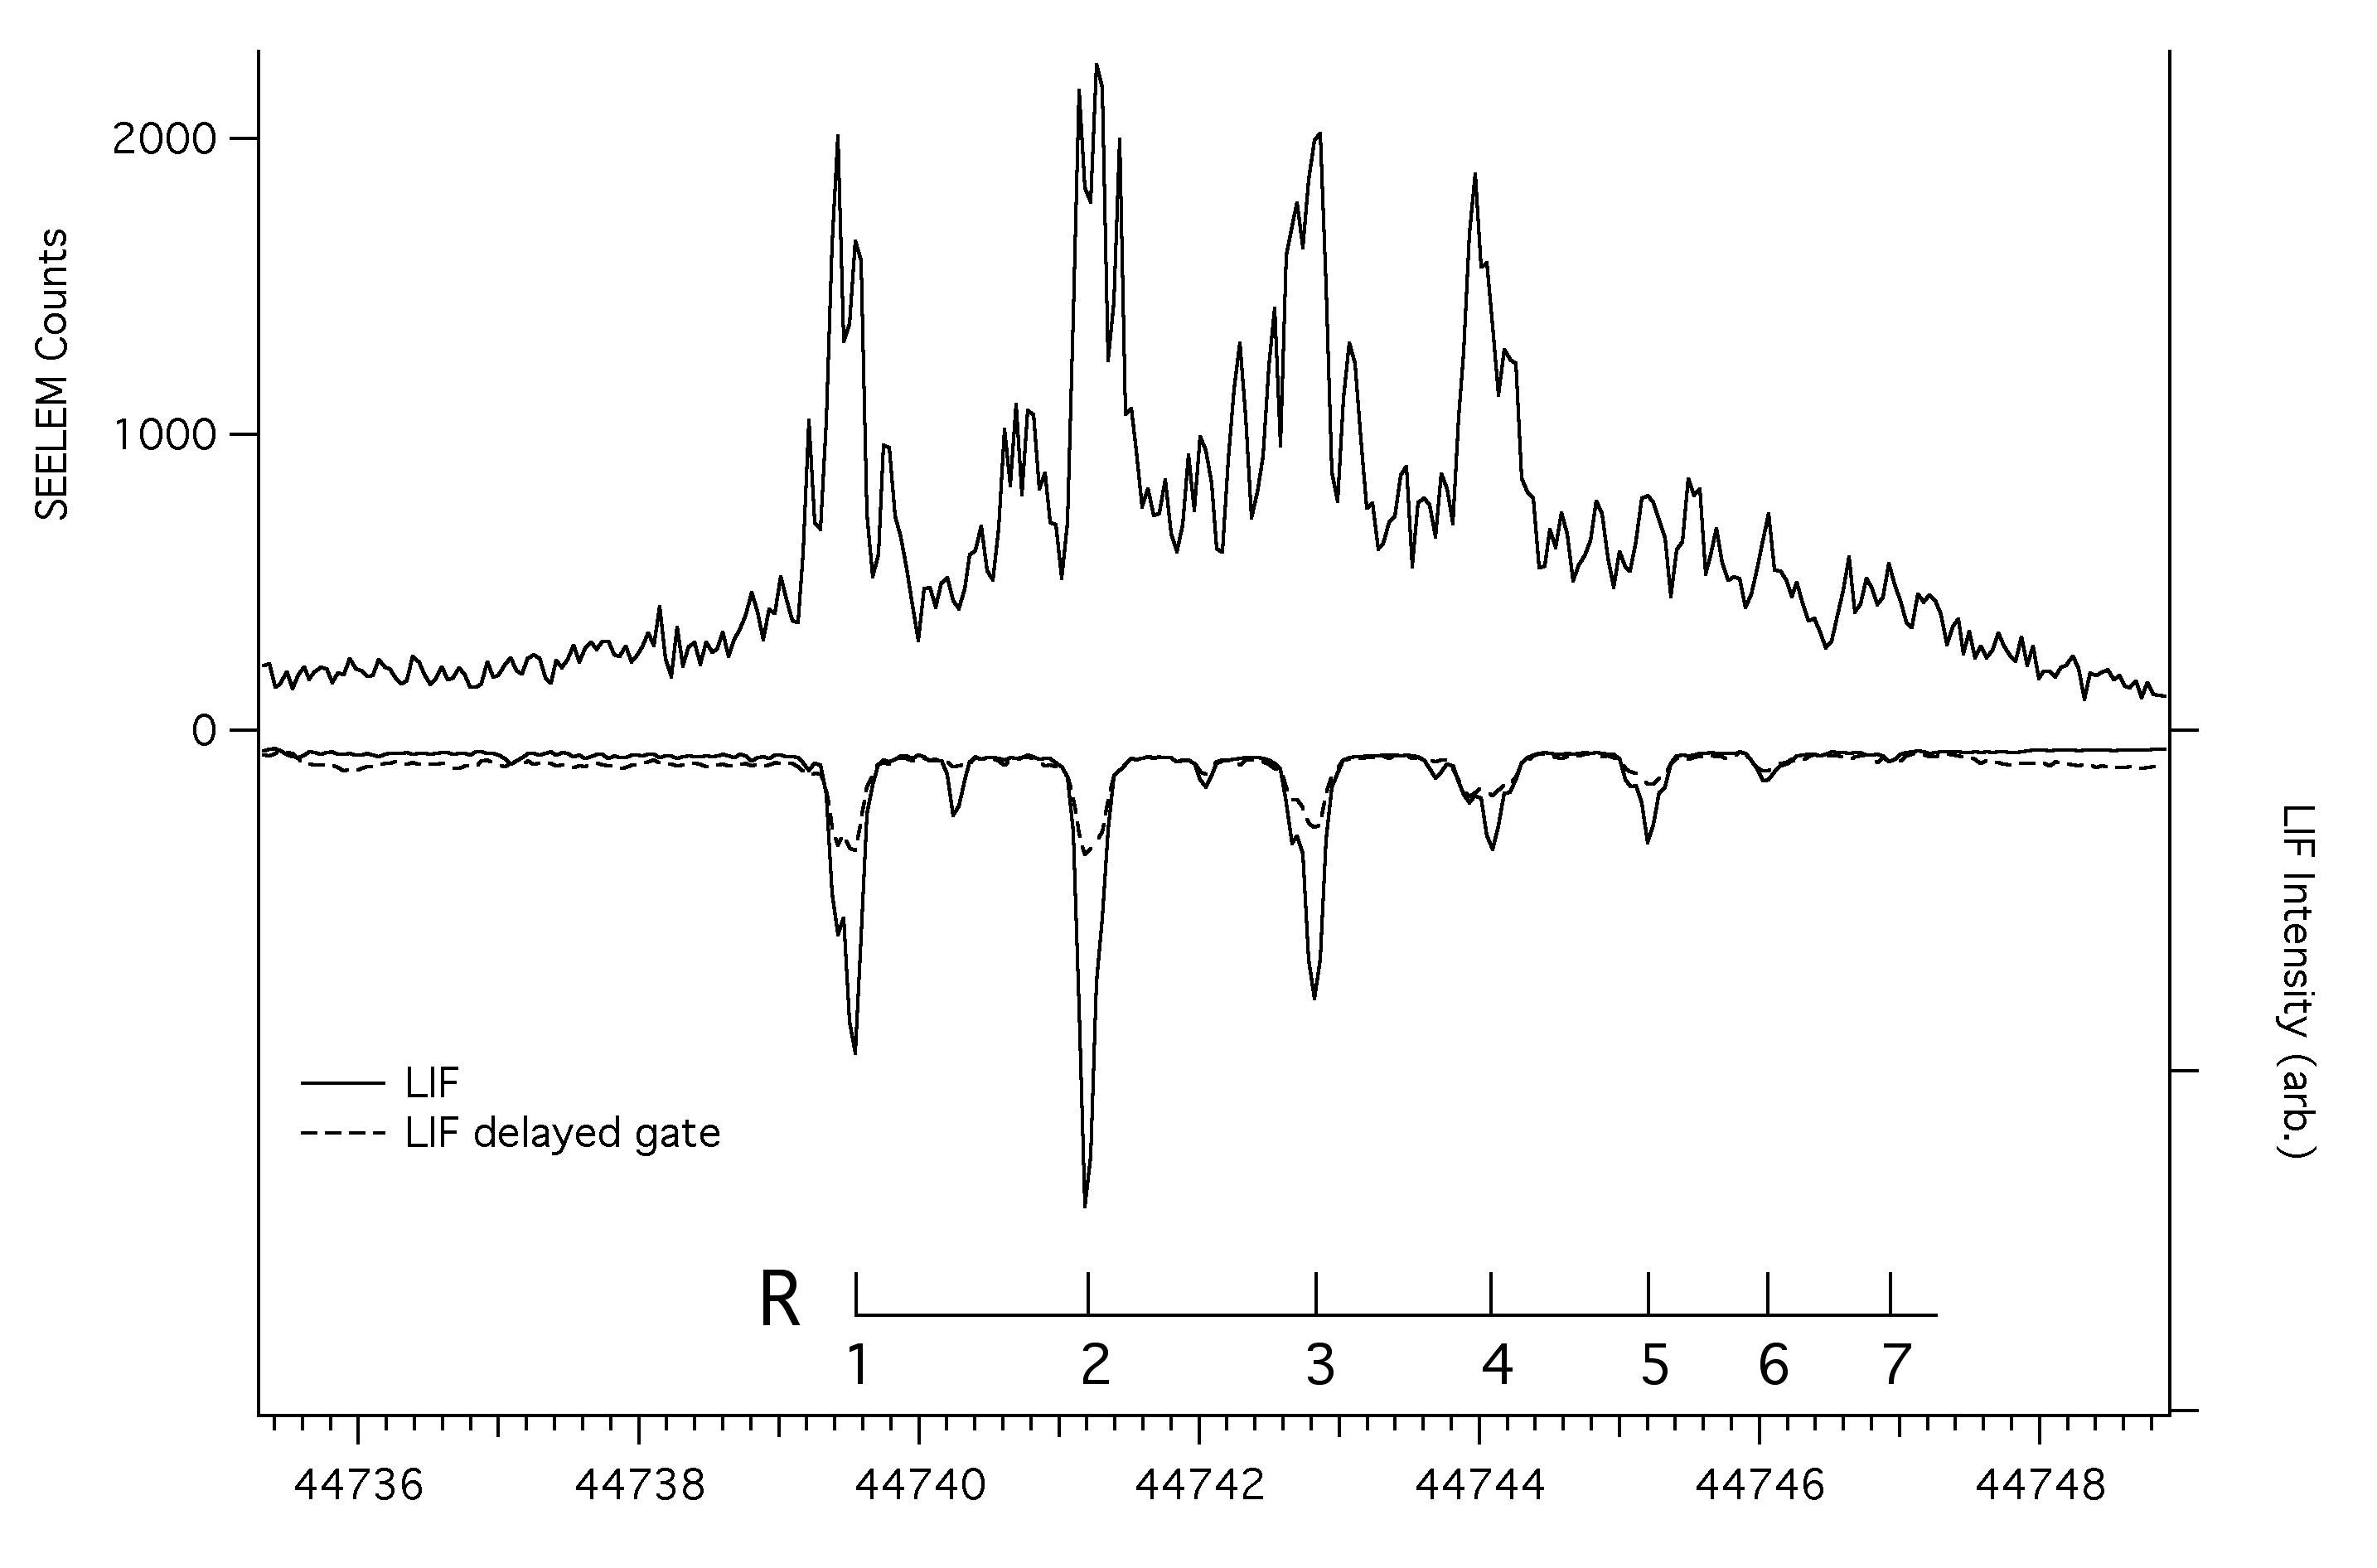
\includegraphics[width=8in,angle=90]{spectrum-33k2.png}
\end{figure}

\TODO{Import calibration points from IGOR.}

Figure \ref{fig:33k2-cog-delay} shows the shifting center of gravity
of a series of rotational lines R(1-7) in the LIF spectrum of the
$3^3$ $K_a$=2 sublevel.

\begin{figure}
  \caption{Shifting center of gravity of a series of rotational lines
    R(1-7) in the LIF spectrum of the $3^3$ $K_a$=2 sublevel.}
  \label{fig:33k2-cog-delay}
  \centering
  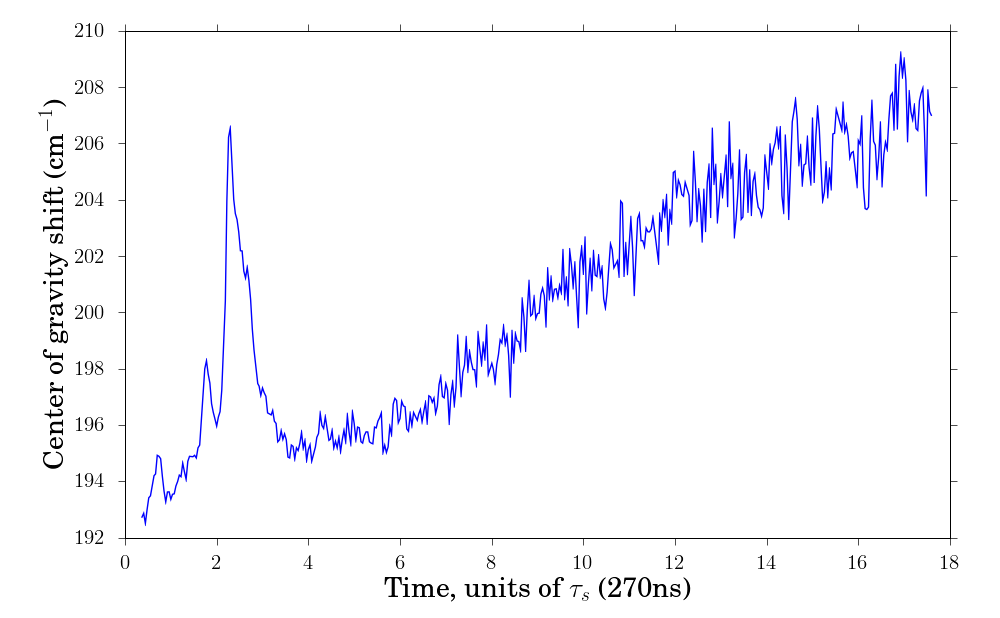
\includegraphics[width=6in]{33k2-cog-delay.png}
\end{figure}

\subsection{The $3^24^2$ $K_a$=1 sublevel}

\POINT{SEELEM spectrum of $3^2 4^2$ with lone SEELEM peak in band gap
  (December 2006, p.86 of 9/2006--1/2007 notebook.)}  This spectrum is
shown in Figure \ref{fig:spectrum-32b2}.

\begin{figure}
  \caption{
    % Simultaneously recorded LIF and SEELEM spectra of the
    % acetylene $V^2_04^2_0K^1_0$ $\tilde{A}^1A_u \leftarrow
    % \tilde{X}^1\Sigma_g$ transition.
    Simultaneously recorded surface electron ejection by laser excited
    metastables (SEELEM, upper trace) and ultraviolet laser-induced
    fluorescence (UV-LIF, lower trace) spectra of the $3^24^2$ $K_a$=1
    sublevel of the $\tilde{A}^1A_u \leftarrow \tilde{X} ^1\Sigma_g^+$
    electronic transition. A delayed, integrated fluorescence signal
    is shown as a dotted trace in the UV-LIF spectrum.}
  \label{fig:spectrum-32b2}
  \centering
  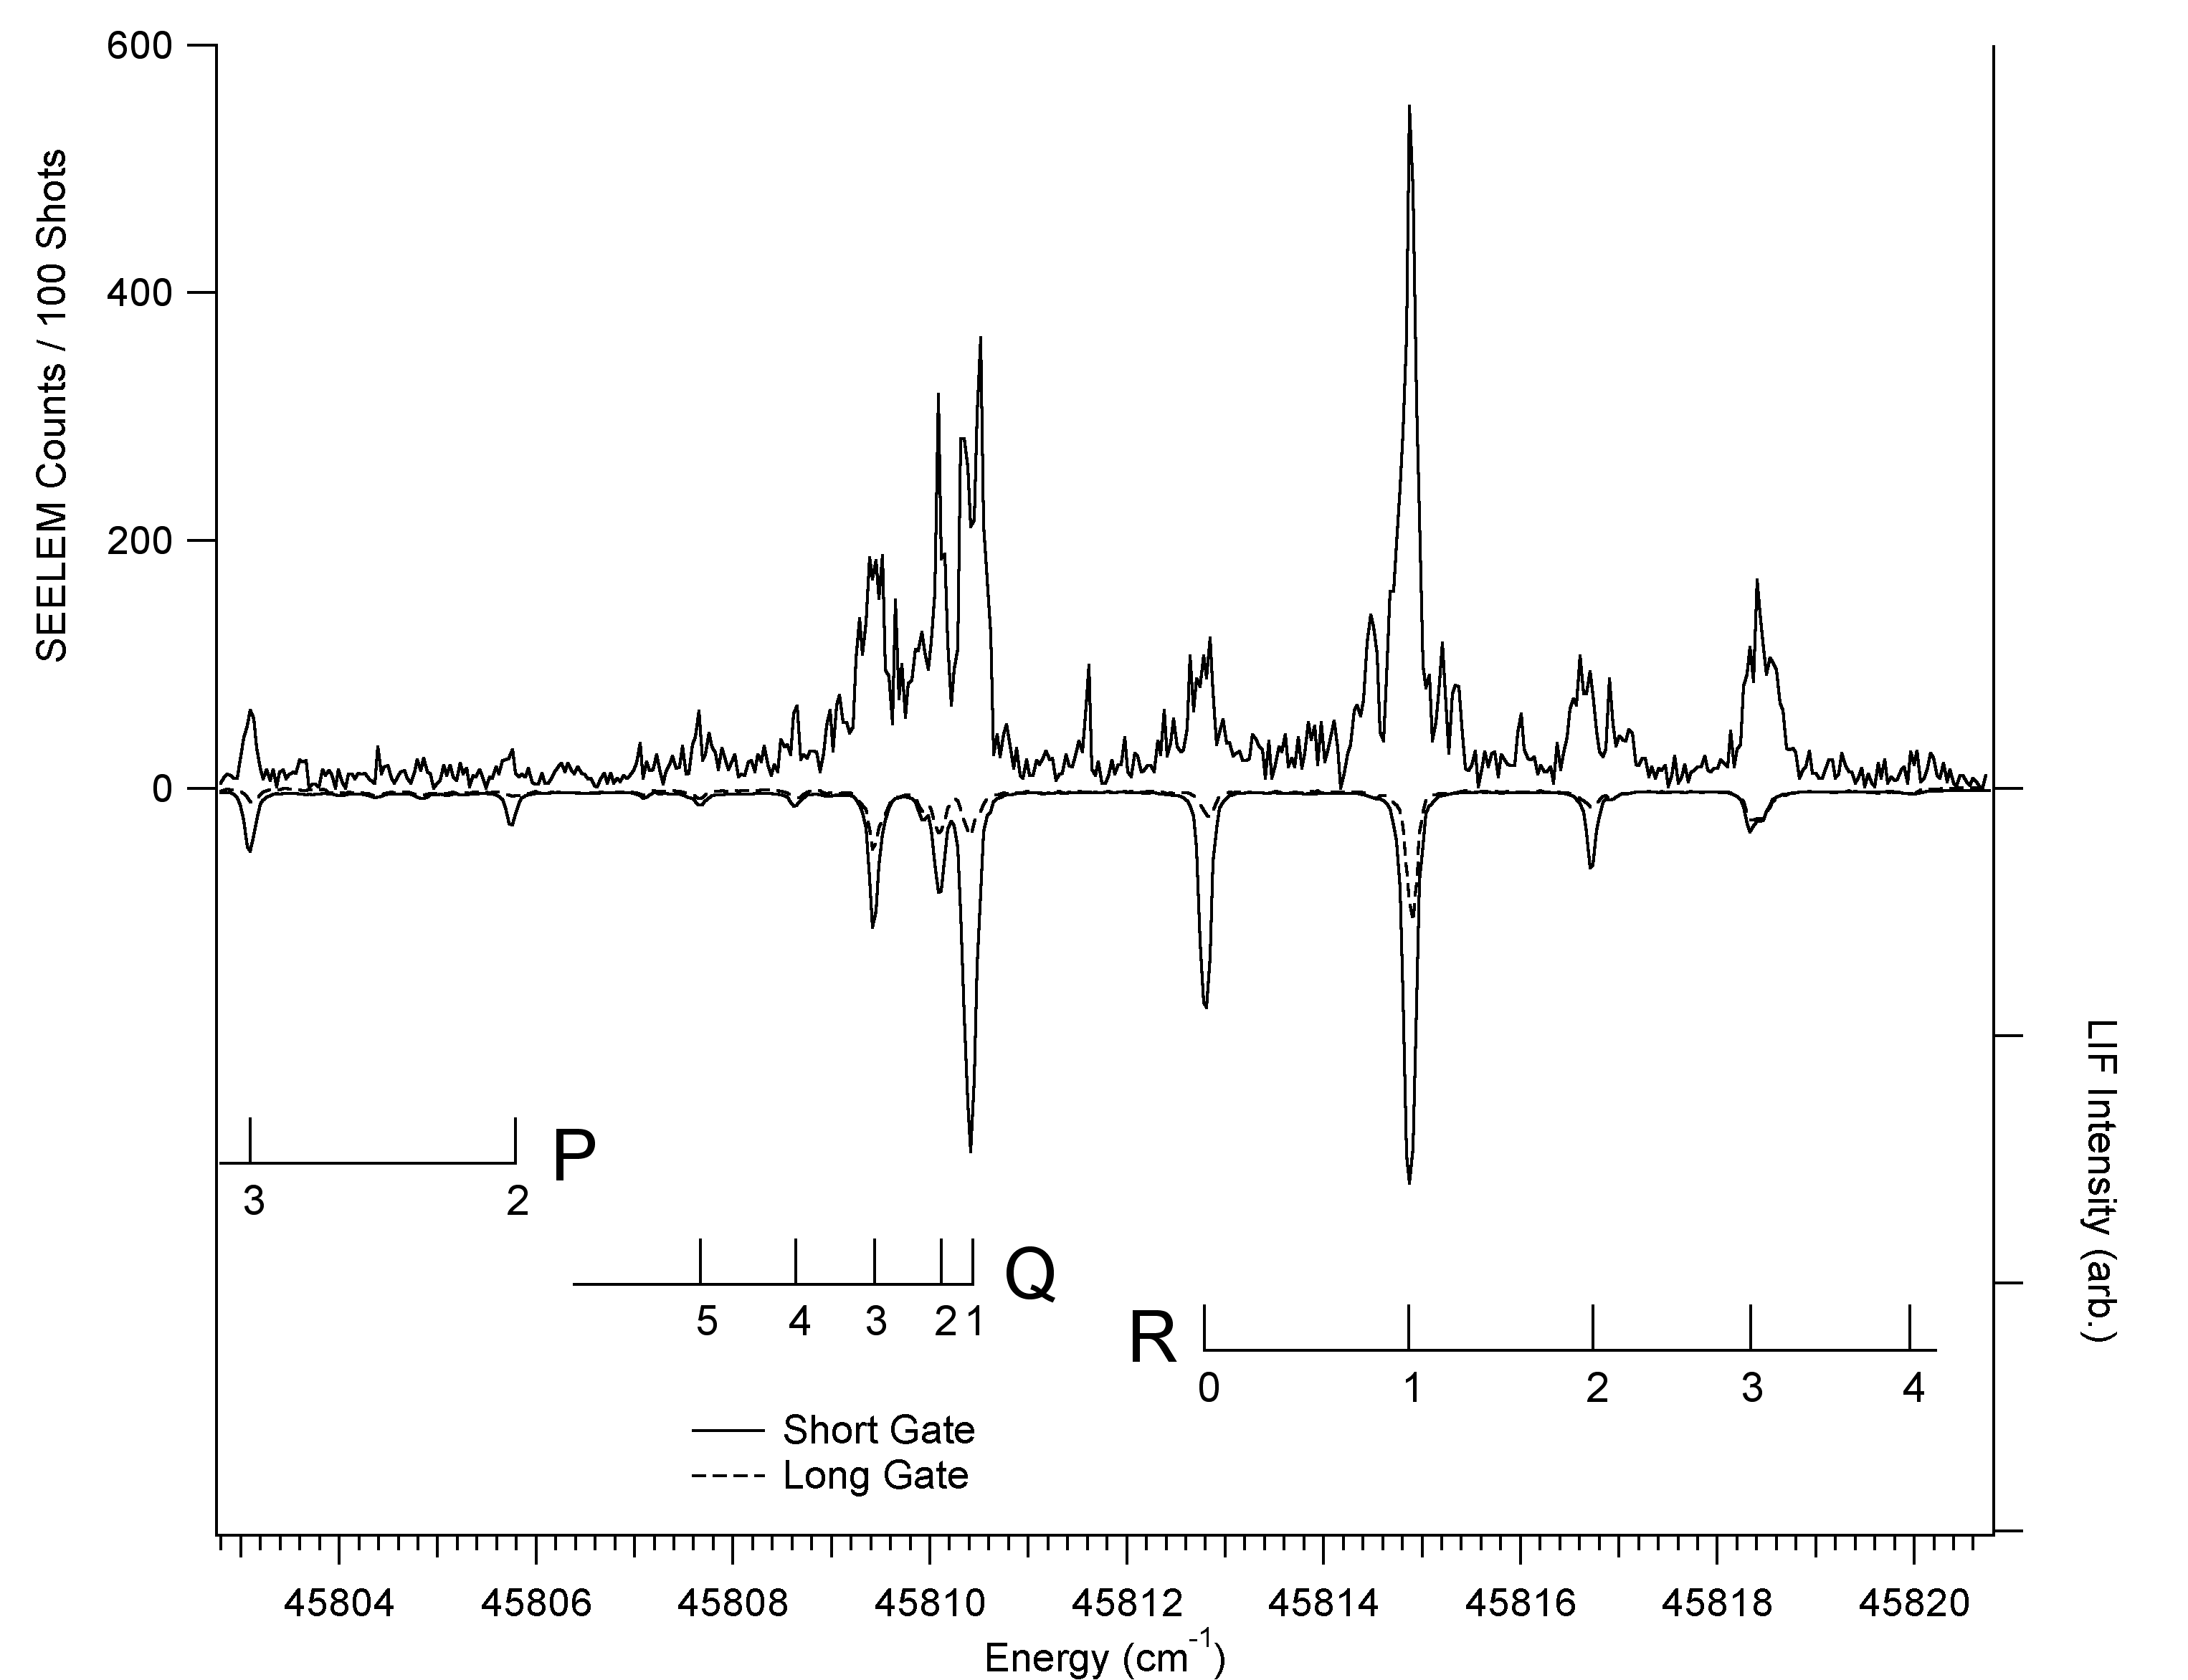
\includegraphics[width=7.5in,angle=90]{spectrum-32b2.png}
\end{figure}

\TODO{Adapt from email.}  Consider the R-branch of this transition.  A
look at the long vs. short gates shows a systematic shift to higher
energy in the delayed (long) gate spectrum.  Here is what happens when
the data is examined using all 500 time divisions available
\ref{fig:32b2-cog-delay}.

\begin{figure}
  \caption{Shifting center of gravity of individual rotational
    lines in the LIF spectrum of the $3^24^2$ $K_a$=1 sublevel.}
  \label{fig:32b2-cog-delay}
  \centering
  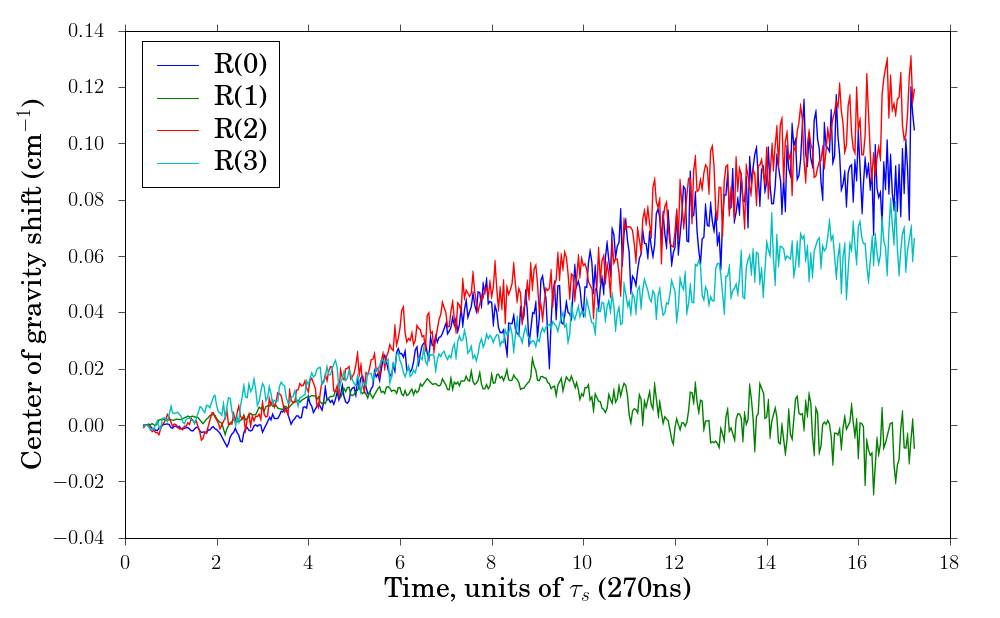
\includegraphics[width=6in]{32b2-cog-delay.png}
\end{figure}

The systematic shift to higher energies at greater time delays is
evident for all the lines, EXCEPT R(1).  In a somewhat peculiar
manner, R(1) begins to shift upward in energy, but then shifts
downward at later times. I believe this to be evidence of a local
perturbation, probably a T3 level which happens to have a small matrix
element with the $3^2 4^2$ level.  (Since the perturbation occurrs
only at $J'$=2, it most likely involves a change in $N$ of $\pm$1 --
see Ryan and Adya's paper for details.)  Looking at the SEELEM
spectrum near the R(1) transition, you'll notice that it is the
strongest feature in the band.  A local $T_3$ perturber which is
fractionated among $T_1$ and $T_2$ levels would explain this strong,
anamolous feature in the SEELEM spectrum.

Although I did not write out the theory for this in my report, I've
also plotted out the variance of the spectral features as a function
of time \ref{fig:32b2-var-delay}

\begin{figure}
  \caption{Shifting variance of individual rotational lines in the LIF
    spectrum of the $3^24^2$ $K_a$=1 sublevel.}
  \label{fig:32b2-var-delay}
  \centering
  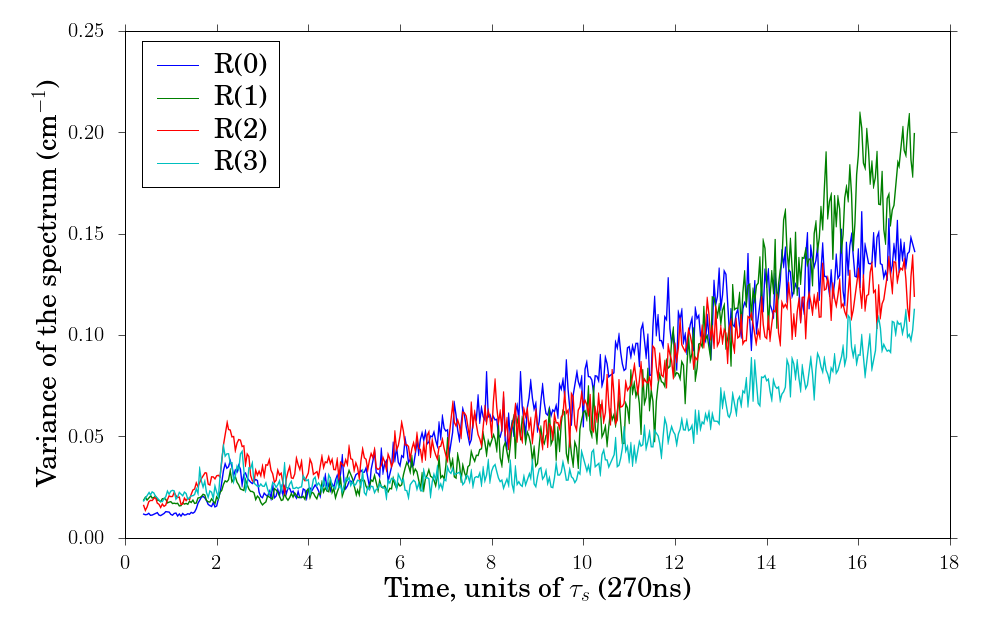
\includegraphics[width=6in]{32b2-variance-delay.png}
\end{figure}

All of the transitions exhibit similar behavior, increasing in
spectral width as our detection method becomes more and more sensitive
to states with smaller amounts of bright state character.  The R(1)
transition may be increasing in variance slightly faster due to the
proposed local interaction, but I hesitate to hang too much weight on
that due to intensity noise.

\section{Discussion}

\TODO{Adapt from email, on the subject of $3^2 4^2$ $K_a$=1.}  The
analysis indicates that the coupling between S1 ($3^2 4^2$) and the
local manifold of T1,2 levels is induced by a non-local mediating
(probably T3) level at higher energy.  If the coupling were
non-mediated, the manifold of T1,2 levels would mix according to their
energy denominators, and we would not observe a systematic shift in
the center of gravity for all transitions in the R-branch.  The
analysis also shows a local perturbation at J'=2.

\TODO{Write this section.}

\section{Conclusion}

The mechanism of doorway-mediated coupling by an energetically distant
$T_3$ level skews the coupling to the local $T_{1,2}$ states appearing
in the SEELEM spectrum, resulting in a center-of-gravity shift between
the LIF and SEELEM spectra.  Additionally, when viewed in successive
time windows, the center of gravity of the LIF spectrum shows a
transition to the limiting behavior exhibited in the SEELEM spectrum.
A simple model can be used to show that strong coupling between the
singlet level and the mediating $T_3$ level causes a gradual shift in
the center of gravity, while weak coupling to the mediating level
induces a more delayed and rapid shift in the center of gravity.

Rotational selection rules for $S_1 \sim T_3$ spin-orbit coupling give
rise to $J$-dependent effects in the LIF/SEELEM spectrum.  As $J$
increases, the $\Delta N$= +1 or -1 components of any distant $T_3$
level approach the singlet at a rate of approximately $2B_T$ (about
2\rcm\ per $J$).  In the spectrum, the result is a shift in the
LIF-SEELEM center of gravity when integrated across an entire branch
of transitions.  The effect not only leads to strong changes in
$T_3$-mediated coupling with rotation, but also ensures "accidental"
$S_1 \sim T_3$ near-degeneracies at relatively low values of $J$.

% \POINT{The LIF/SEELEM spectra for the progression of $2^n3^m$ levels
%   shows the expected trends for strong coupling.}

The universality of triplet perturbations via $F_1$ and $F_3$
components of $T_3$ levels in the spectrum of acetylene ensures that
further LIF/SEELEM spectroscopy of the \astate\ state will be fruitful
and informative.  Primary candidates for further investigations are
(1) levels exhibiting long lifetimes or quantum beats in the LIF
spectrum, (2) levels with unassigned perturbations or splittings, (3)
other $3^2B^2$ polyad members, (4) other $K$-sublevels of the
Franck-Condon active levels studied here.

\bibliography{master}
\bibliographystyle{plain}
\end{document}




President's Report:

The T_3 electronic state is peculiar among the valence states of
acetylene due to its out-of-plane equilibrium geometry. One of the
most interesting unsolved problems in the intersystem crossing of
acetylene is the role of the non-symmetric in- and out-of-plane S_1
bending modes (\nu_4 and \nu_6) in promoting coupling to the nonplanar
T_3 state.  To investigate this issue, we have used an IR-UV-Double
Resonance technique to record simultaneous LIF/SEELEM spectra of the
3^3 4^1 K=0 and 3^3 6^1 K=0 levels.  This method allows us to record
the spectrum of weakly coupled T_1,2 levels without overlap from
adjacent rotational transitions.

[Additionally, we have used a polarization technique in tandem with
IRUVDR to record the spectrum of the rotationless level in 3^3 6^1
K=0.  Due to spin-orbit selection rules, only triplet levels having
K_T = J_T = N_T = 0 may appear in the spectrum -- thus, the local
T_1,2 level density may be obtained from a direct count of SEELEM
transitions.]


That should be K_T = J_T = 0 and N_T = 1...my bad. For a K=0 triplet
level in Hund's case (b),

N            J

  ---------- 3
2 ---------- 2
  ---------- 1


  ---------- 2
1 ---------- 1
  ---------- 0  ***


0 ---------- 1

--Kyle



The total spin-orbit matrix element between a rovibronic level of S_1
and a level of T_3 is the product of an electronic factor, a
vibrational overlap factor, and a rotational factor (arising from
angular momentum coupling laws).

OK, these are kind of hairy, but hold on before you start to panic.
As it turns out, the energy differences between levels of S_1 and T_3
vary much more rapidly than the rotational factors.  This is due to
the spin-orbit selection rule of \Delta_N = 0, +1, -1.

Take a look at this plot: It shows the relative energies of the three
triplet rotational components that are connected to singlet level: F_1
(\Delta_N = -1), F_2 (\Delta_N = 0), and F_3 (\Delta_N = +1).  This
plot is made in the approximation that the singlet and triplet
B-values are nearly equal.  Imagine placing a singlet level at some
energy on the plot - the energy of the singlet could be represented by
a horizontal line.  If the singlet is very close to zero, the F_2
component varies slowly with rotation and the F_1,2 components rapidly
speed away.  Essentially, only the F_2 component matters when J>1.

If the singlet is not located close to zero, EITHER the F_1 or the F_3
component of the triplet is rapidly approaching.  The triplet
component approaches with a rate of about 2 cm-1 per rotational
quantum number. According to Ryan and Bryan's calculations, the
<electronic*vibrational> spin-orbit matrix elements between S_1 and
T_3 max out at about 0.1 cm-1. The rotational factor only reduces this
value.  Compared to the matrix element, an energy difference of 2 cm-1
per J is huge!

I believe that strongly coupled, mediating T_3 levels will make
themselves known at several values of J through this
energy-denominator effect.  I think this is what we observe in our 3^3
K=2 data.  Weakly coupled T_3 levels should appear as perturbations at
a single J, and then immediately disappear, because their matrix
elements are much, much less than 2 cm-1. This means that weak triplet
perturbations should be _common_, and it means that we should be able
to infer their approximate energy from the value of J which is
perturbed in the singlet, i.e. + or - (J*2*B).

This means that further SEELEM spectroscopy of the S_1 state should be
fruitful and informative.  I hope you are all totally stoked!  I'll
discuss the experimental consequences and possibilities in a later
email.

--Kyle
